%%%%%%%%%%%%%%%%%%%%%%%%%%%%%%%%%%%%%%%%%%%%%%%%%%%%%%%%%%%%%%%%%%
%  Thesis template file  prepared by:
%  Thyge Knüppel, tkn@elektro.dtu.dk, DTU Elektro, May 2008
%  Based on the work of Jan Larsen, IMM, DTU (cf. http://www2.imm.dtu.dk/teaching/phd/)
%
%  CET June 2010 edited Charlotte K. Madsen
%%%%%%%%%%%%%%%%%%%%%%%%%%%%%%%%%%%%%%%%%%%%%%%%%%%%%%%%%%%%%%%%%%

%%%%%% Compilation: 
% compilation using latex (i.e. via a ps file)
\documentclass[a4paper,11pt,oneside,openright,dvips]{book}

% compilation using PDFLATEX - Note that pdflatex is known to have issues with
% some of the pstricks-packages
% 	\documentclass[a4paper,11pt,twoside,openright,pdftex]{book}
%%%%%%%%%%%%%%%%%%%%%%%%%%%%%%%%%%%%%%%%%%

%%%%%%%%%%%%%%%%%%%%%%%%%%%%%%%%%%%%%%%%%%%%%%%%%%%%%%%%%%%%%%%%%%
% Input information for cover, titlepages:
% Sould be EDITED to match your work!

%multiple authors separated by "\\"
%If there are multiple authors adjust the \vspace 
%in thesislayout.sty as necessary 
\def\ThesisAuthor{Mads Lundt, s103439 \\
			      Matthias Larsen, s103437 \\
			      Joachim Jensen, s103430}
			      
%list of authors for pdf
%properties. Multiple authors separated by ","
\def\ThesisAuthorForHyperref{Mads Lundt, s103439 , Matthias Larsen, s103437 , Joachim Jensen, s103430}

%project title
\def\ThesisTitle{Weather data visualization}

%subtitle - if any
\def\Subtitle{A Graphical User Interface (GUI) for weather radar and wind energy data visualization and analysis} 

%keywords for the pdf file
\def\thesiskeywords{Software Technology Project, Weather data visualization} 

%only for pdf properties - doesn't appear on printed versions
\def\thesissubject{}

%list of supervisors. multiple supervisors are separated by "\\"
\def\Supervisor{Pierre Pinson//Pierre-Julien Trombe} 

%type of project (see README file %for explanation)
\def\projecttype{Software Technology Project, June 2012} 

%type \ISBNNUMBER{ISBN: xxx} if your project has one
\def\ISBNNUMBER{} 

%date of publication
\def\DatePublished{June, 2012} 

%project class (see README file for explanation)
\def\Klasse{1 (public)} 

%obtained degree (see README file for explanation)
\def\Degree{Master of Science in Engineering (M.Sc.Eng.)} 

%# of ECTS points 
\def\ECTSpoints{10} 

%edition
\def\Udgave{First} 

 %name of copyright and year
\def\Owner{Mads Lundt, Matthias Larsen, Joachim Jensen, 2012}
%%%%%%%%%%%%%%%%%%%%%%%%%%%%%%%%%%%%%%%%%%%%%%%%%%%%%%%%%%%%%%%%%%

%%%%%%%%%%%%%%%%%%%%%%%%%%%%%%%%%%%%%%%%%%%%%%%%%%%%%%%%%%%%%%%%%%
%%%%%%%%%%%%% Change settings: (compile twice )%%%%%%%%%%%%%%%%%%%%%%
%OBS: choose this for final version (official set of title pages) 
\def\thesisversion{final} 
%OBS: choose this for working-copy draft version (simple title page and no info page)
%\def\thesisversion{workingcopy} 
%OBS: choose this for draft version (offical title pages, no info page and water marked)
%\def\thesisversion{draft} 
%OBS: choose this for draft version (simple title page /w logo)
%\def\thesisversion{majorassignment}
%OBS: choose this for draft version (only simple title page /w logo)
%\def\thesisversion{minorassignement}  
                         

%\def\thesislinks{no}%OBS: choose this for paper version (no colored links) 
\def\thesislinks{yes}%OBS: choose this for online version (with links)
%%%%%%%%%%%%%%%%%%%%%%%%%%%%%%%%%%%%%%%%%%%%%%%%%%%%%%%%%%%%%%%%%%

%%%  For changing language: (compile twice -first time gives errors)%%%
\def\thesislanguage{en} %OBS: compile document for English 
%\def\thesislanguage{da}  %OBS:  compile document for Danish


%%%%%%%%%%%%%%%%%%%%%%%%%%%%%%%%%%%%%%%%%%
% Load style definitions, packages, etc:
	\usepackage{style/thesisdef} 		% packages  listings aso
	\usepackage{style/thesislayout} 	% layout; headings, pagemargin, theorems aso
	\usepackage{style/mathboxes}		% example and other math boxes
	\usepackage{style/Mythesis} 	  	% Locals editings to only your thesis
%%%%%%%%%%%%%%%%%%%%%%%%%%%%%%%%%%%%%%%%%%
% END of premable
%%%%%%%%%%%%%%%%%%%%%%%%%%%%%%%%%%%%%%%%%%%%%%%%%%%%%%%%%%%%%%%%%%

%%%%%%%%%%%%%%%%%%%%%%%%%%%% DOCUMENT %%%%%%%%%%%%%%%%%%%%%%%%%%%%
	\begin{document}

%%%%%%%%%%%%%%%%% Edit ONLY for printing type:
% Front matter:
	\frontmatter

  \ifx\thesisversion\printversion
	% for final version include standard dtu cover pages
	\pagenumbering{alph}%dummy numbering for pdf-file (numbering set as a
                    %pdf-property and is NOT visible on the document). The
                    %hyperref package complains if duplicate numbering exists
	\coverpages    %generates the first four pages (thesislayout.sty)
	\else
%for draft version use simple title page:
	\title{\ThesisTitle{} - \Subtitle{}}
	\author{\ThesisAuthor}
	\thispagestyle{empty}
	\maketitle
	\clearpage{\thispagestyle{empty}\cleardoublepage}
   \fi
%%%%%%%%%%%%%%%%%%%%%%%%%%%%%%%%%%%%%%%%%%

%%%%%%%%%%%%%%%%%%%%%%%%%%%%%%%%%%%%%%%%%%%%%%%%%%%%%%%%%%%%%%%%%%
% PREFACE CHAPTERS INCLUDE: files are in folder "file"
	%\pagestyle{empty} 	%For first few pages %\markboth{}{}
	
%% Ad to List of Contents:
\chapter*{Acknowledgements}
%The solutions provided by this report to the Weather data visualization -- A Graphical User Interface (GUI) for weather radar and wind energy data visualization and analysis, has been developed by Mads Lundt ($s103439$), Matthias Larsen ($s103437$) and Joachim Jensen ($s103430$).

We would like to express our gratitude to Pierre Pinson and Pierre-Julien Trombe for giving us the opportunity to work on this project.

Morten H. S. Jespersen for his assistance in the layout of the paper.

Especially, we would like to give a special thanks to Adam L. Baxter for proofreading this paper.
	
\pagenumbering{roman}
  \ifx\thesisversion\printversion % no resumes in draft-version
%% Ad to List of Contents:
\chapter*{Abstract, Resumé}
	\ifx\thesislanguage\danishlang
	\addcontentsline{toc}{chapter}{Resumé}
	\else
	\addcontentsline{toc}{chapter}{Abstract}
	\fi
% State the problem, your approach and solution, and the main contributions of the paper. Include little if any background and motivation. Be factual but comprehensive. The material in the abstract should not be repeated later word for word in the paper.
Data for weather analysis and forecasts consists of enormous amounts of data.

To predict the weather, a lot of variables is in play including wind speed, pressure and tendency.

Comparing huge amounts of data quickly becomes hard. Most people interprets images easier than numbers, hence the need for some sort of visualization for the data sets.

Today no free application exists for visualizing the weather data except for two earlier attempts: one in MATLAB and one with Google Maps. These earlier application were not flexible enough to be used in bigger context.

This report shows the development and considerations throughout the project of an application that might serve as the beginning of a new common open source platform for analyzing, visualizing and comparing weather related data.
\todo[inline]{Abstract / Resume}
\fi
%% Ad to List of Contents:
%\chapter*{Resumé, Abstract}
%	\ifx\thesislanguage\danishlang
%	\addcontentsline{toc}{chapter}{Abstract}
%	\else
%	\addcontentsline{toc}{chapter}{Resumé}
%	\fi
%\input{file/resume}
%  \fi
% if a chapter is wanted BEFORE lists
%% Ad to List of Contents:
%\chapter*{Preface, Forord}
%	\ifx\thesislanguage\danishlang
%	\addcontentsline{toc}{chapter}{Forord}
%	\else
%	\addcontentsline{toc}{chapter}{Preface}
%	\fi
%\input{file/preface} %lines above can be moved into this file
%%%%%%%%%%%%%%%%%%%%%%%%%%%%%%%%%%%%%%%%%%%%%%%%%%%%%%%%%%%%%%%%%%

%%%%%%%%%%%%%%%%%%%%%%%%%%%%%%%%%%%%%%%%%%
% TOC,LOF,LOT and SETUP HEADER: (should not be edited)
	%\pagestyle{fancyplain}		%'plain' enable center-food-pagenumber only
							%'fancyplain' gives right-left numbers

	\cleardoublepage 	\phantomsection  	% makes pdf-hyperref work in adobe
	\ifx\thesislanguage\danishlang
	\addcontentsline{toc}{chapter}{Indhold}
	\else
	\addcontentsline{toc}{chapter}{Contents}
	\fi
\tableofcontents  

  \ifx\thesisversion\printversion	
	\cleardoublepage 	\phantomsection  	% makes pdf-hyperref work in adobe
	\ifx\thesislanguage\danishlang
	\addcontentsline{toc}{chapter}{Figurliste}
	\else
	\addcontentsline{toc}{chapter}{List of Figures}
	\fi
\listoffigures

	\cleardoublepage 	\phantomsection  	% makes pdf-hyperref work in adobe
	\ifx\thesislanguage\danishlang
	\addcontentsline{toc}{chapter}{Tabelliste}
	\else
	\addcontentsline{toc}{chapter}{List of Tables}
	\fi
\listoftables
  
  	\cleardoublepage 	\phantomsection  	% makes pdf-hyperref work in adobe
	\ifx\thesislanguage\danishlang
	\addcontentsline{toc}{chapter}{Kildekode liste}
	\else
	\addcontentsline{toc}{chapter}{List of Source code}
	\fi
\lstlistoflistings
  \fi
%%%%%%%%%%%%%%%%%%%%%%%%%%%%%%%%%%%%%%%%%%

\label{fancy:frontend} %for 'of page /x'
\clearpage{\thispagestyle{empty}\cleardoublepage}

%%%%%%%%%%%%%%%%%%%%%%%%%%%%%%%%%%%%%%%%%%%%%%%%%%%%%%%%%%%%%%%%%%
% MAIN CHAPTERS INCLUDED FROM FOLDER  "file":
	\mainmatter %\setcounter{page}{1}\pagenumbering{arabic} if mainmatter fails

% if a chapter is wanted after lists or other unnumbered chapter
%% Ad to List of Contents (can also be the first entry after \chapter in the file:
	\cleardoublepage 	\phantomsection  	
	\ifx\thesislanguage\danishlang
	%\addcontentsline{toc}{chapter}{Introduktion}
	\markboth{Forord}{}
	\else
	%\addcontentsline{toc}{chapter}{Introduction}
	\markboth{Preface}{}
	\fi
	
\listoftodos

\renewcommand{\nomname}{List of Notations}

\makenomenclature
\nomenclature{$a$}{The number of angels per unit area}%
\nomenclature{$N$}{The number of angels per needle point}%
\nomenclature{$A$}{The area of the needle point}%
\nomenclature{$\sigma$}{The total mass of angels per unit area}%
\nomenclature{$m$}{The mass of one angel}
\printnomenclature

\chapter{Introduction}
\label{sec:introduction}

% The Introduction is crucially important. By the time a referee has finished the Introduction, he's probably made an initial decision about whether to accept or reject the paper -- he'll read the rest of the paper looking for evidence to support his decision. A casual reader will continue on if the Introduction captivated him, and will set the paper aside otherwise. Again, the Introduction is crucially important.

% Here is the Stanford InfoLab's patented five-point structure for Introductions. Unless there's a good argument against it, the Introduction should consist of five paragraphs answering the following five questions:

% What is the problem?
The problem with this project is analysing the different kinds of data and visualize it in a smooth and easy way. There are other weather applications on the market, but one of the requirements to create the new weather application, is using open source (OpenStreetMap, Qt etc.). We had different kinds of data in different languages, CSV-files, WRK-files and NC-files. We only did the implementation for CSV-files and WRK-files.\\
We are very focused on getting high performance and getting this optimized - that was one of the biggest challenges.

% Why is it interesting and important?
This is interesting because there is a lot of data to analyse and visualize, and still want\todo[fancyline,color=green]{Adam: Mangler et subjekt} high performance and user-friendly overview. There have been combined different programming language to get it optimized. All this and still it should be functional and user-friendly.

% Why is it hard? (E.g., why do naive approaches fail?)
This is tough, because there had to be some changes during its construction, such as implement database integration, to get this optimized. Many of these changes are to satisfy our own requirements through the project.\\
There are a lot of data to analyse and visualize, so there has be figured out how to do this in the best possible way.

% Why hasn't it been solved before? (Or, what's wrong with previous proposed solutions? How does mine differ?)
There are other applications out there, like DMI and TV2-vejret, but none of these satisfied our requirements that was specified at the beginning. DMI had many different data, but wasn't created in a user-friendly way and TV2-vejret only have weather forecast. There are similar weather programs out there, but none of these have either user-friendly way of handling huge amount data or using open source.

% What are the key components of my approach and results? Also include any specific limitations.
\todo[inline]{What are the key components of my approach and results? Also include any specific limitations?}

% Then have a final paragraph or subsection: "Summary of Contributions". It should list the major contributions in bullet form, mentioning in which sections they can be found. This material doubles as an outline of the rest of the paper, saving space and eliminating redundancy.
\chapter{Requirements}
We stated some requirements to the final product, that should be fulfilled. 
The requirements:
\begin{itemize}
\item Web based software using opensource software.
\item Upload data to server in seperate files and compressed files.
\item Analyse and read data from CSV, WRK and NC-files.
\item Visualize the data in a nice user-friendly way.
\item Several performance requirements
\end{itemize}
We created the web based software using opensource.\\
It is allowed to upload CSV, WRK and zip-files.\\
We didn't do the implementation for the NC-files, because of difficulty and time pressure. However, CSV and WRK-files are working just fine, even if they both are compressed into one zip-file.\\
The visualizing of data are done in very user-friendly and cool design. We used a lot javascript, to create this cool and user-friendly design.\\
The performance is very good and the server is doing the most work, so even computers with poor specifications can access. We have done some caching\footnote{A collection of data duplicating original values stored on the server or by the client's web browser}, to get better performance too.\\

\section{Application requirements}
\label{sec:application_requirements}
The application requires a few things in order to run.
\begin{description}
\item[Web server] A web server is needed in order to run the web site. It is also required to have permissions to run executables. The included data parser is compiled for Windows, OSX and Ubuntu. If the web server is not allowed to run the included executables, they should be ran as a CGI script - This has not been tested however.
\item[PHP] The web server should support PHP version 5.3+.
\item[GD] The application uses GD 2.0.1+ (2.0.28+ is recommended) to create radar images.
\item[MySQL] FuelPHP supports multiple databases through drivers, but in order to support time zones correctly, we've chosen to take advantage of MySQLs own methods. This means that MySQL 5.5.20+ is required.
\item[Zoneinfo] MySQL needs Zoneinfo in order for the time zones to work properly\footnote{On linux, the following command can be executed in the terminal to import zoneinfo: \mbox{\textsf{> mysql\_tzinfo\_to\_sql /usr/share/zoneinfo | mysql -u root -p mysql}}. Other operating systems might not have the zoneinfo, and will have to download it from \url{http://dev.mysql.com/downloads/timezones.html} and import it to the mysql database.}
\item[Safe mode] Safe mode might need to be disabled in the PHP configuration, if \textsc{fopen}\footnote{See \url{http://php.net/manual/en/function.fopen.php}.} is not allowed to access some files.
\end{description}
\chapter{Analysis}
A lot of considerations has gone into the development process of the application. The following chapter explains the considerations with the most impact on the application.

\section{Comparison}
It's been discussed if it should be possible to compare data from multiple wind farms at the same time, and how it should be done if that was the case.

One of the ideas was to let single click on a windmill put it in a `selected' state and a double click on a windmill would trigger the comparison view between all the windmills in the `selected' state.

The comparison view was also discussed to be either one chart, like the one implemented, but with all the data represented with different colors for each wind farm.
Another way of viewing them was to have multiple small draggable windows, each one representing a wind farm. This would allow browsing the data for each wind farm independent of each other, but also make it annoying when wanting to compare the same time and having to manually move forth or back in time on each window.

We chose to drop comparison because we fell short of time, but the above ideas could be used to develop some sort of comparison of data from multiple sources at the same time.

\section{Radar annotation}
In the final stages of the application, it was discussed if radars should have its name and/or time stamp for the current radar image shown.

Figure \ref{fig:mock_up_inactive_radar} and \ref{fig:mock_up_active_radar} shows the mock ups for the radar in both inactive and active state.
\begin{figure}[htbp]
  \begin{minipage}[b]{0.5\linewidth}
    \centering
    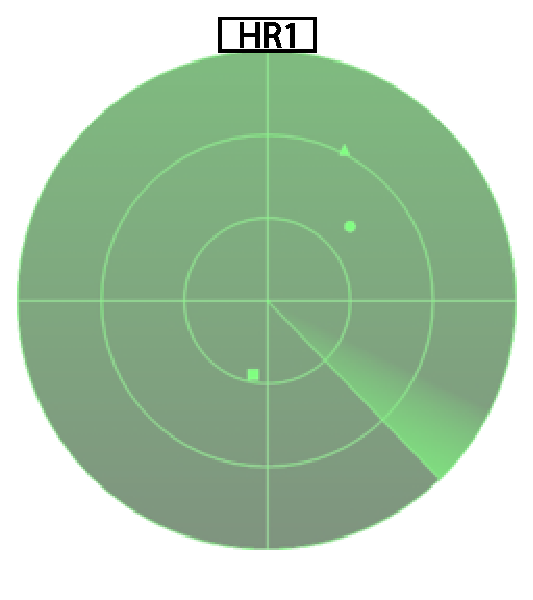
\includegraphics[width=\linewidth]{figure/radar1.eps}
    \caption{Mock up of inactive radar}
    \label{fig:mock_up_inactive_radar}
  \end{minipage}
  \hspace{0.5cm}
  \begin{minipage}[b]{0.5\linewidth}
    \centering
    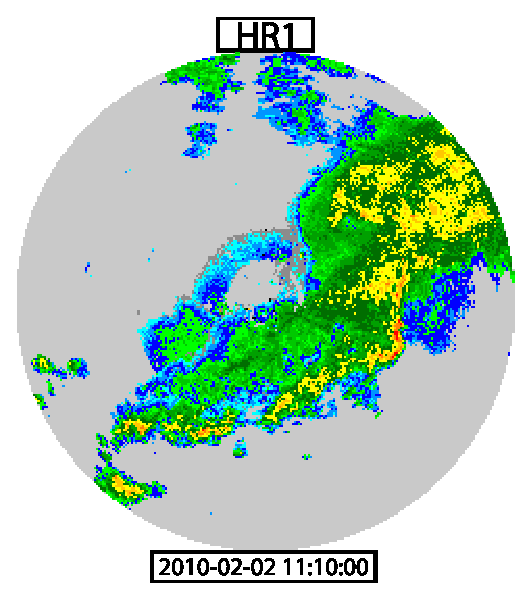
\includegraphics[width=\linewidth]{figure/radar2.eps}
    \caption{Mock up of active radar}
    \label{fig:mock_up_active_radar}
  \end{minipage}
\end{figure}
The added name and time stamp might pose as a problem, if two radars were placed in such a way that their range would overlap where the name or time stamp were put.

This could be somewhat solved, by fading out the radars too close to an active radar, in the same way that windmills inside the range of a radar is faded out when a radar animation starts.

\section{Data date range}
As time goes by, one would expect the application to contain massive amounts of data.
In the provided test data\footnote{Data02122.tar.gz provided by Pierre-Julien Trombe on CampusNet}, the application contains \textasciitilde 140 rows of data for \textsf{wrk} files and \textasciitilde 73,000 rows of data for the wind farm data.

It was discussed how we should limit the view of data, since it would require quite a lot of processing power to display that much data.

For the wind farm chart, we went from 1-month, weekly and daily view to 2-week, weekly and daily.
Preliminary tests showed that the loading time for 1-month view was too slow, because of the huge amount of data that had to be processed and formatted correctly before sent to the browser. The data would also take long to download, especially if not on a high speed internet connection.

Another problem was the radar images. Without any data range, they would all start at the first image taken by that radar, and play till the last. A range chosen by the user from a `to' and `from' date field was suggested. After testing the first implementation it was found that the `to' field was a bit confusing and would result in a bit of a rewrite of already existing code.

The `to' field was removed and the `from' field now decides the starting date for all radars and wind farm charts.
All radars will start their animation on the first image taken after the selected from date.
The chart will also start at the selected start date, but the navigation buttons allows one to go either back or forth in time independent of the selected from date.

\section{Radar interaction}
A lot of considerations went into the interaction of the radars. The primary focus of the radar design was to make it intuitive.

A `play' button to start animation of all radars were considered, but after a test implementation it was found to give a weird feeling and was removed again.

All radars will play after a single click and pause the animation if click while an animation is running. A double click will reset the radar to the first image and display the image for an inactive radar.

\section{The data}
\subsection{Implementation}
The massive amount of data forced a prioritized list of the order of which the data types should be implemented.

After a quick look at the data, it was decided that the data from the wind farm was the first one to be implemented due to its simplicity.

Research showed that the wrk file was in a relatively easy format with decent documentation\footnote{See \cite{VRIS} for the documentation}, where as the NetCDF\footnote{Network Common Data Form - See \cite{netcdf}} format was very complex with little documentation\footnote{A framework for the file type was found but with very little documentation}.

After the implementation of wrk files, it was discussed whether or not the NetCDF should be implemented and it was decided that the time cost were too big to meet the deadline. Instead it was concluded that the flexibility of the application was good enough to allow extending the application to support other file formats, including NetCDF, at a later date and the focus was shifted to the frontend.

\subsection{Grouping wrk}
The big amount of wrk files for each radar (1 every \textasciitilde 10 minutes for a total of 144 files per day) causes a bit of confusion in the file administration of the control panel.

It was suggested that the administration panel grouped the wrk files per day, or that the data parser combined one day of wrk files into one file before importing it into the database.

The idea of letting the data parser to handle the merge was dropped due to the complexity. A merge in the data parser would also increase the memory usage by the data parser, which might not be available on the web server running the application.

Lack of time prevented the implementation of file grouping by the administration panel because of the work involved in finding the files that should be grouped together.

\subsection{Choice of map}
There were two obvious map options - OpenStreetMap and Google maps. We know Google maps from Google, Facebook, etc.. The previous weather project were using Google maps, so at the beginning it was obvious that we were going to use Google maps.

\begin{figure}[htbp]
\begin{tabular}{| l | l | l |}
\hline
& \textbf{OpenStreetMap} & \textbf{Google maps} \\
\hline
\textbf{Price} & Free & Commercial price \\
\hline
\textbf{View} & Standard & Standard, satellite and street view \\
\hline
\multirow{1}{*}{\textbf{License}} & Anyone can edit. & Owned by multiple organisations.  \\ & Open source & Data is copyrighted \\ & (``CC BY-SA'') & (``NAVTEQ'' / ``TANA'') \\
\hline
\textbf{API} & Yes & Yes \\
\hline
\end{tabular}
\caption{Comparing OpenStreetMap and Google maps}
\end{figure}

After comparing the two maps, it quickly became OpenStreetMap. It was partly because of Google wants money if the map is used for commercial purposes and because the data is copyrighted and owned by multiple organisations. This wasn't the way we were thinking about open source.

OpenStreetMap wasn't that difficult to work with, due to the very well documentation from leaflet\footnote{See \cite{leaflet} for the documentation}.

There have been several design ideas. Many changes through the project and many considerations.
\subsubsection{Map}
At the beginning we had a sidebar which could be visible or hidden (figure \ref{fig:map_v1}). Later we found out that there is no need for a big menu, so we removed the sidebar and added a tiny top bar, with only the necessary options.\\
First mockup:
\begin{figure}[htbp]
   \centering
   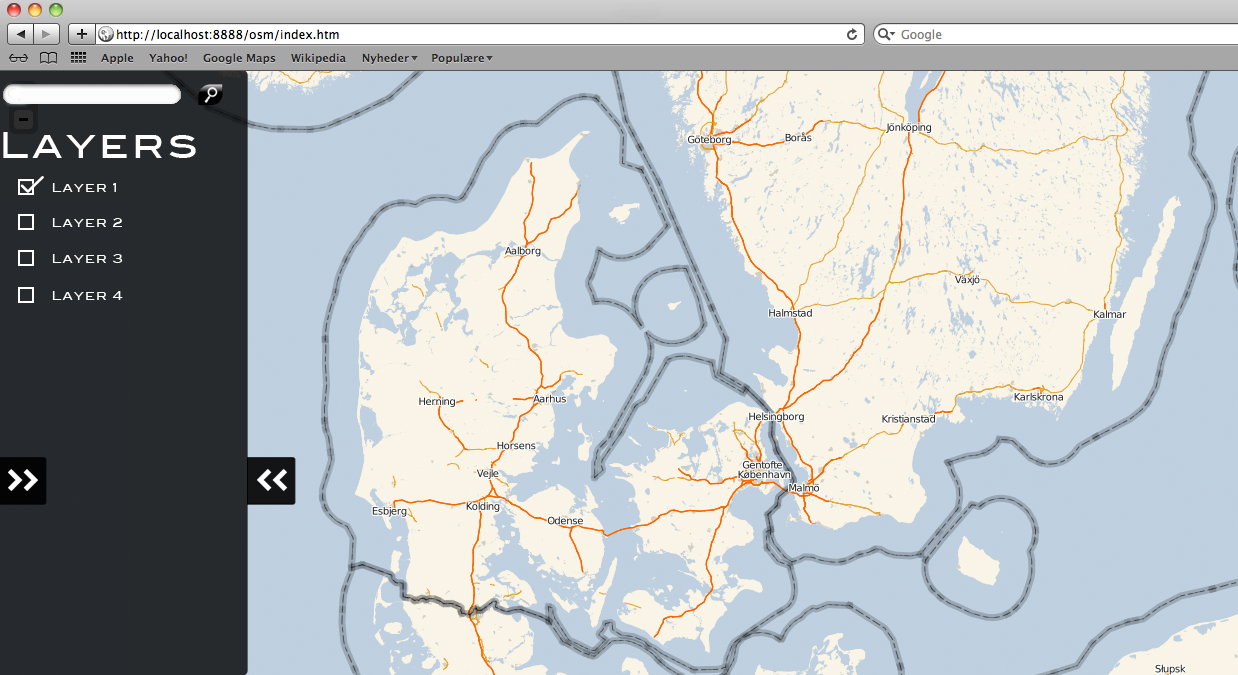
\includegraphics[scale=.3]{figure/design_map_v1.eps}
   \caption{Map - version 1}
   \label{fig:map_v1}
\end{figure}

We would like to have different layers on the map at the beginning, but this was unnecessary, so it was quickly removed.\\
Now we have created a cool design which is easy to get used to and all relevant informations can be accessed easily and without to much clicking (figure \ref{fig:map_final}).
There have also been added some gestures to control the radar easily.\\
The top bar has a date field to know which date the radar should get data from. This date will be transferred to the chart window.

\begin{figure}[htbp]
   \centering
   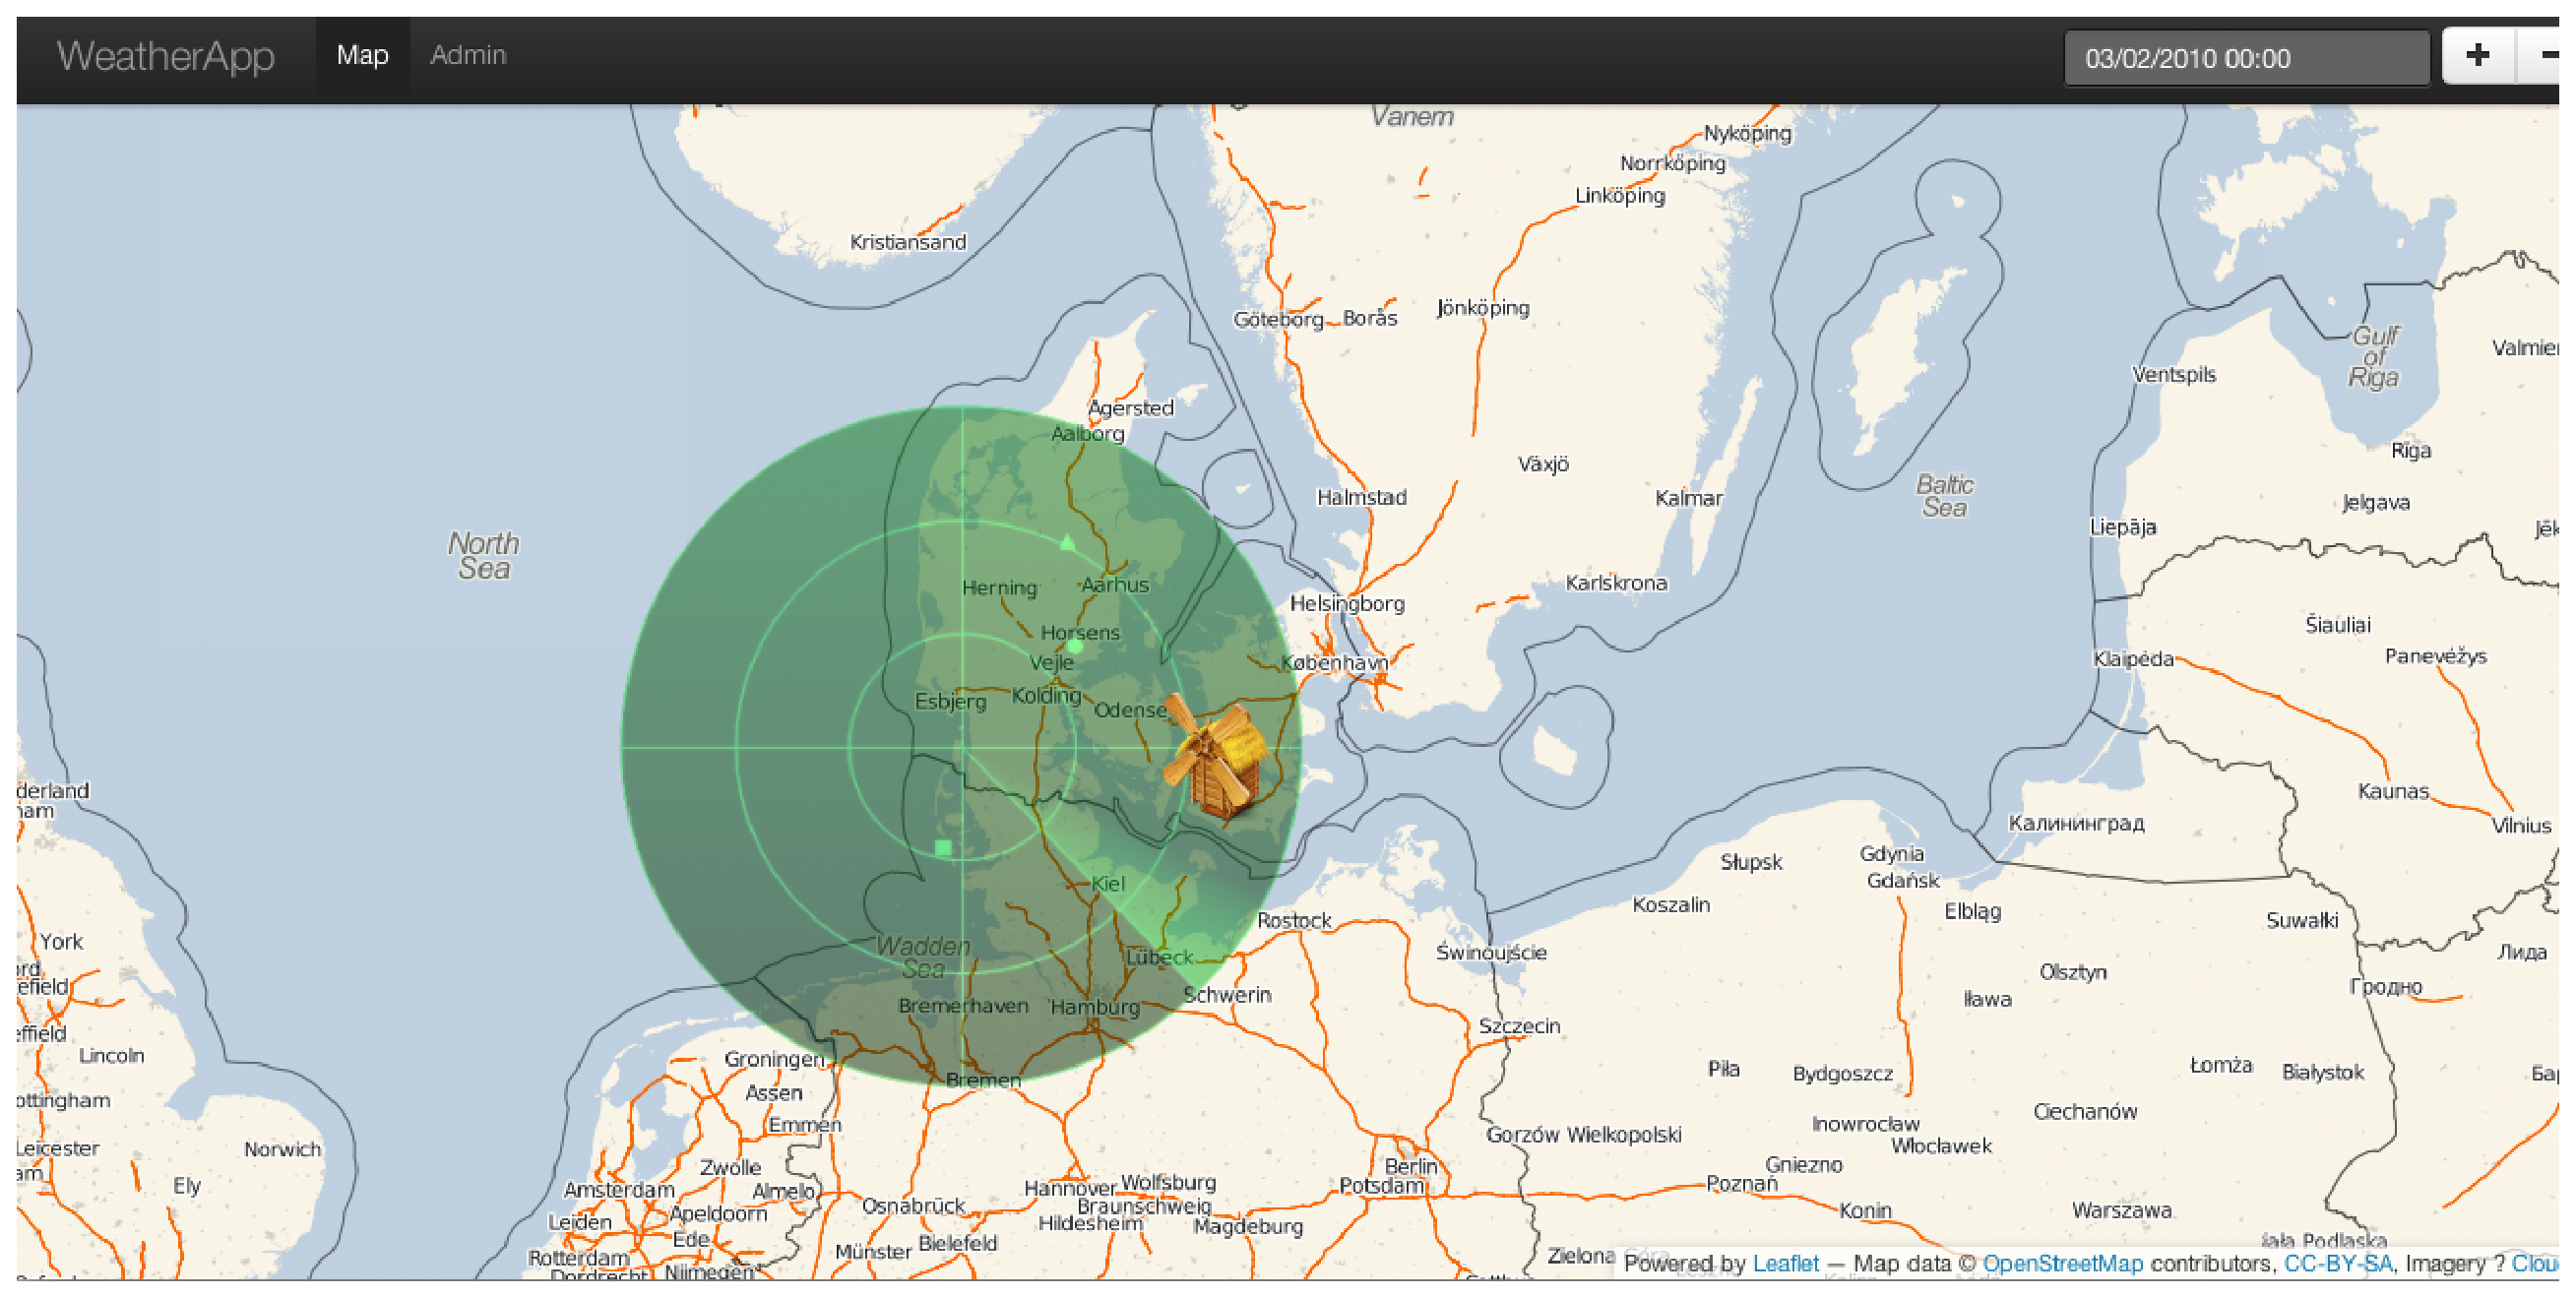
\includegraphics[width=1\linewidth]{figure/design_map_final.eps}
   \caption{Map - final}
   \label{fig:map_final}
\end{figure}

\subsubsection{Chart}
At the beginning we had the same sidebar as on the map, but with other options (figure \ref{fig:chart_v1}). This was also replaced by a top bar like on the map.\\
First mockup: 
\begin{figure}[htbp]
   \centering
   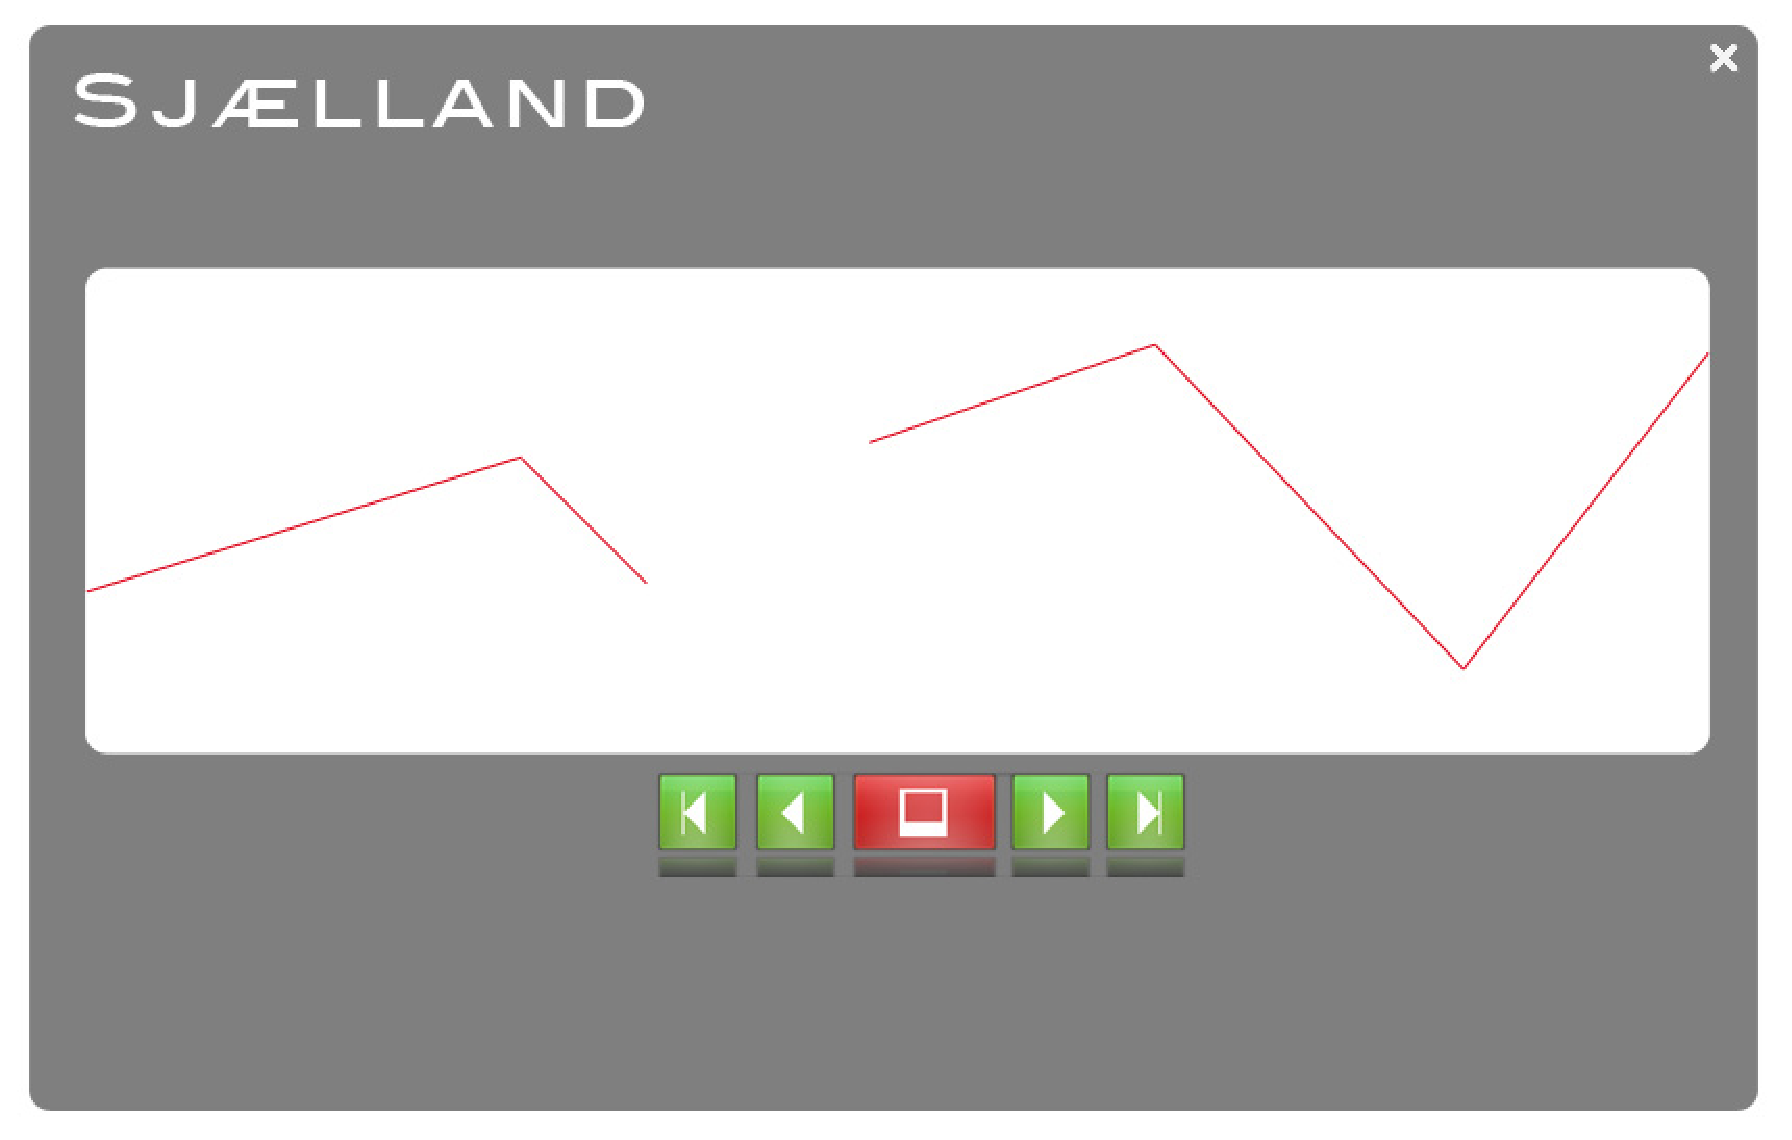
\includegraphics[width=1\linewidth]{figure/design_chart_v1.eps}
   \caption{Chart pop up - version 1}
   \label{fig:chart_v1}
\end{figure}

This has, through the whole project, been determined to be a pop up on the map.
The control buttons were before 'fast backward', 'backward', 'today', 'forward' and 'fast forward', but 'today' was replaced with 'play'. The 'play' button moves the chart every second, so the user can view the chart animated.\\
The new design also have three different views '2-week', 'weekly' and 'daily view' (figure \ref{fig:chart_final}). Control buttons adjust to the view the user has selected.

\begin{figure}[htbp]
   \centering
   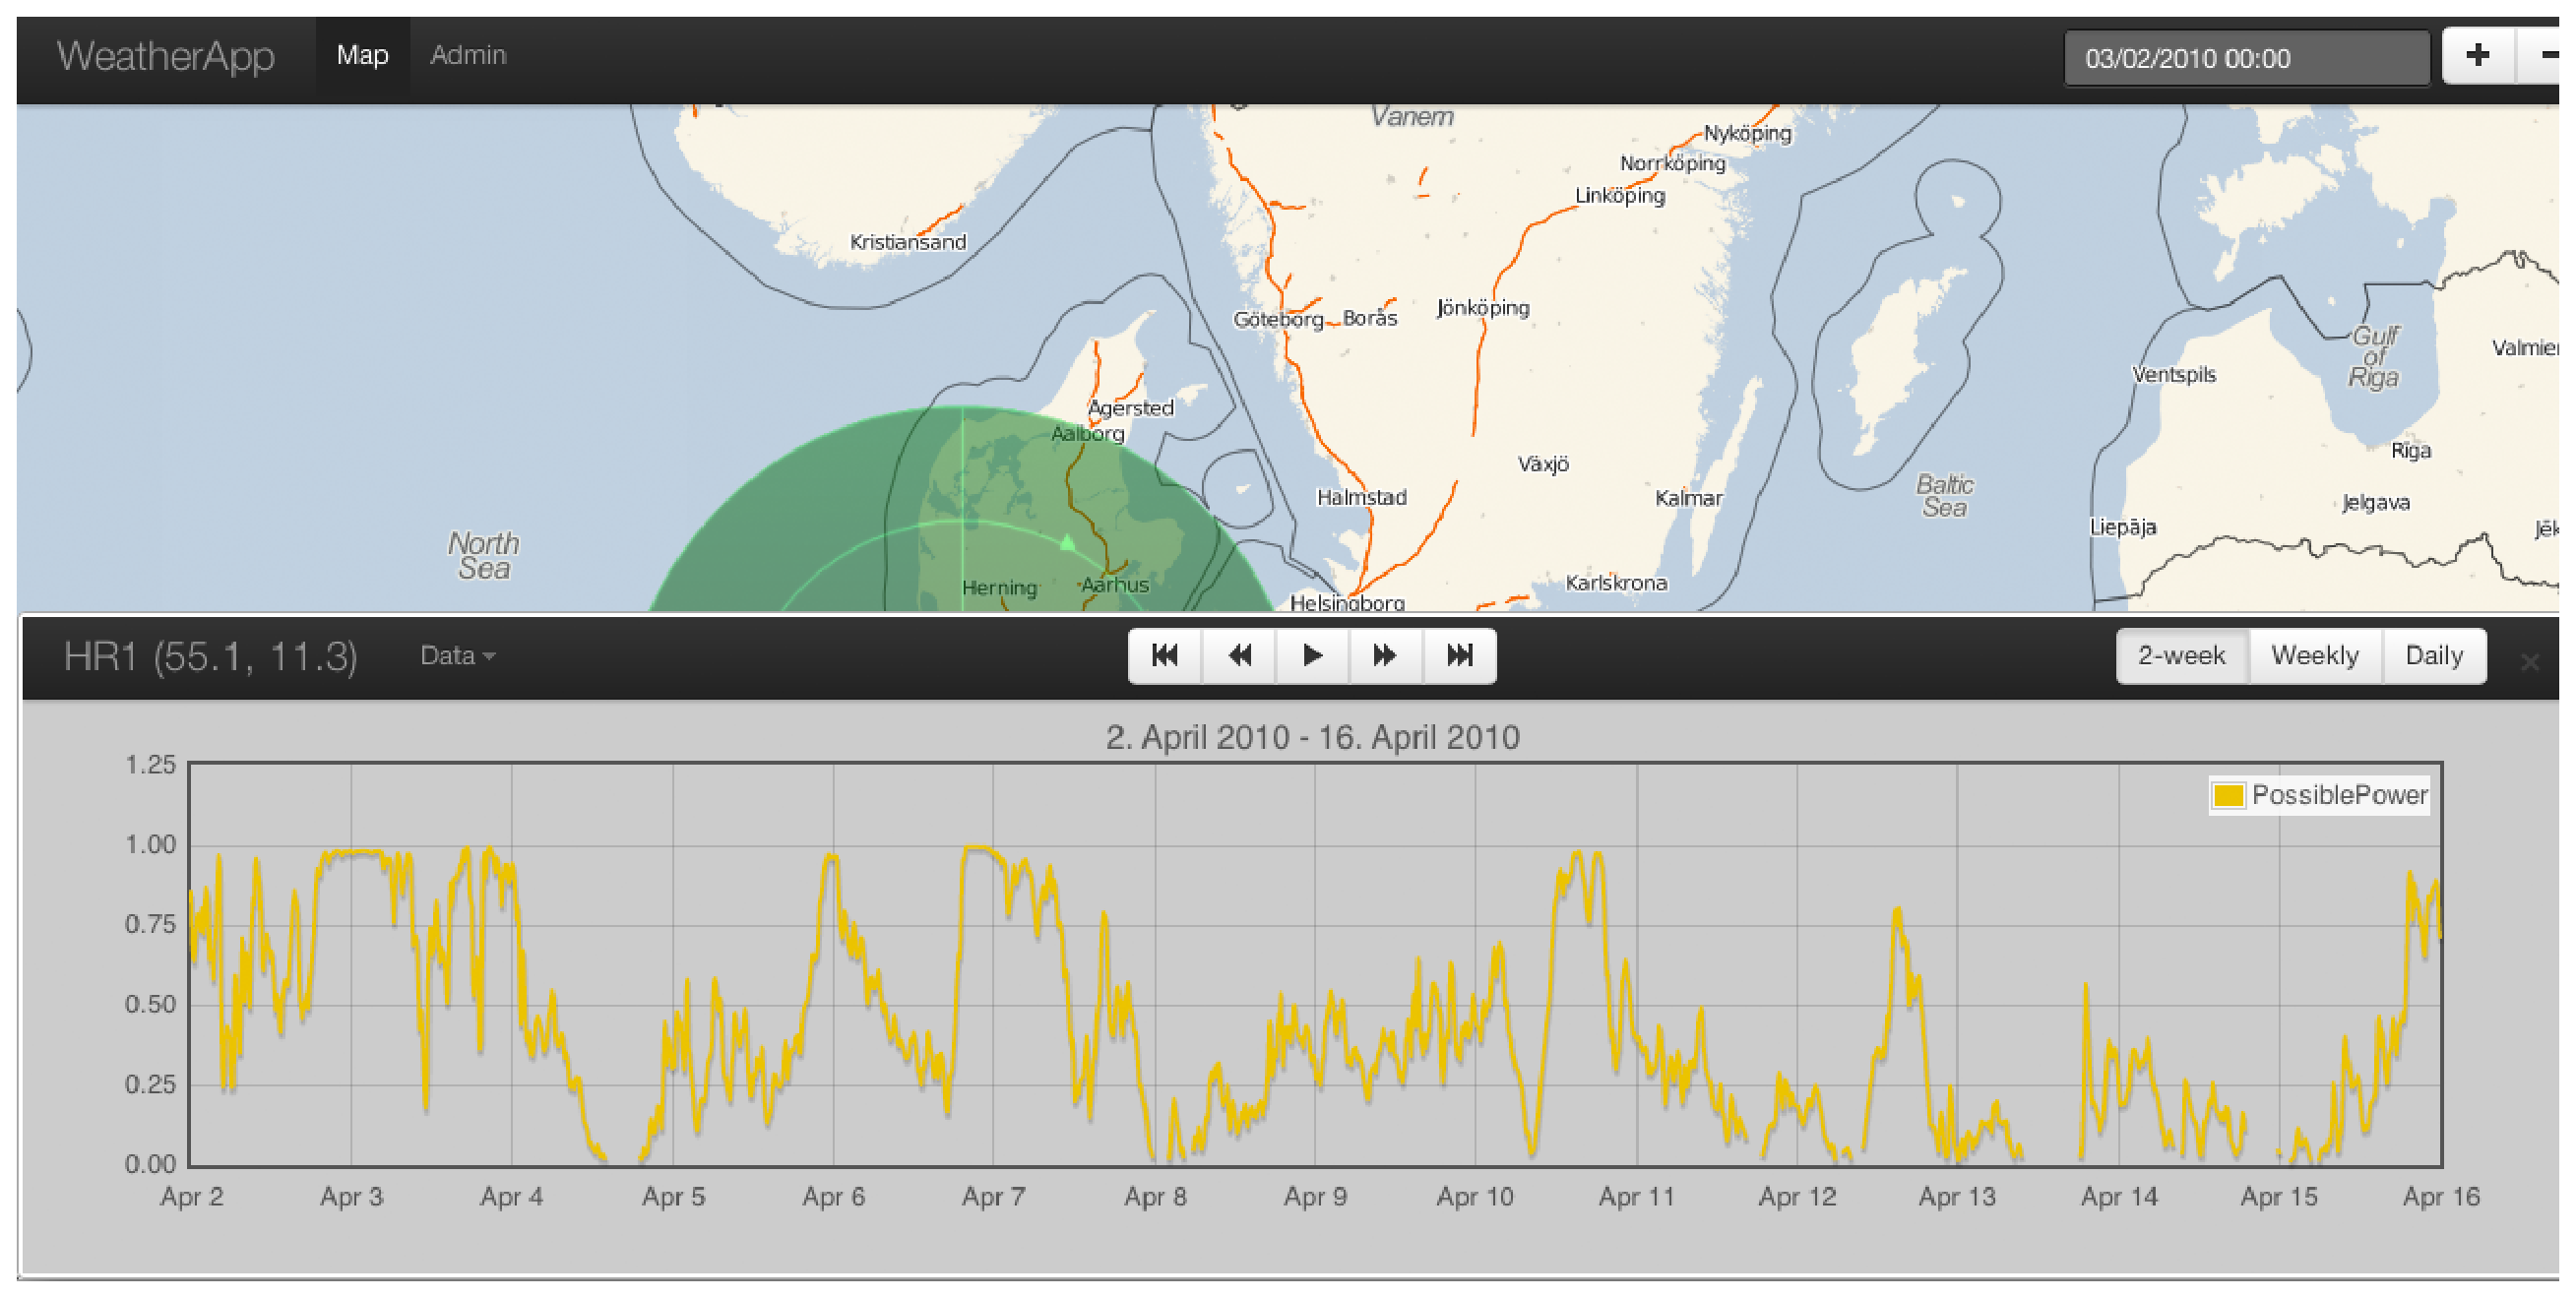
\includegraphics[width=1\linewidth]{figure/design_chart_final.eps}
   \caption{Chart pop up - final}
   \label{fig:chart_final}
\end{figure}

\chapter{Design \& Implementation}
\section{The use of frameworks}
Using frameworks because of the decreased development time due to already developed and tested libraries for various tasks such as database accesss, file handling and file uploading.

\section{Backend}
\subsection{The C++ application}
\subsubsection{Why a C++ application?}
We're using a C++ application because it is much faster to parse huge files in C++ than PHP or JavaScript.
The choice of language was because we had some knowledge of both C and C++. C++ is object oriented where as C is a procedural language, and seeing as we all favour object oriented programming, the choice between the two was easy.

We could have chosen other languages such as F, F\#, Java, Perl or Ruby, but our limited knowledge about these made us stick with C++, which is also quite fast and portable.

\subsubsection{Why Qt?}
We've decided to use Qt because of the support and community around it. It's very mature and most importantly, object oriented.

Qt is a cross-platform application framework developed by Nokia. Popular software such as Skype, VLC media player and VirtualBox along with companies as Google, HP, Philips and Samsung uses it.

Qt makes developing an application with a GUI\footnote{Graphical User Interface} relatively easy, but we've opted to only use the command line part of Qt, because the programming is run by the application and not by a user.

\subsubsection{Return codes}
The PHP part of the application gets a return code from the C++ application depending on how the parsing went and reacts accordingly. A list of the return codes can be seen in table \ref{tab:cppReturnCodes}.
\begin{table}[htbp]
\centering
\begin{tabular}{|l|l|}
\hline
\textbf{Code} & \textbf{Explanation}\\
\hline
0 & Failure\\
\hline
1 & Success\\
\hline
2 & Success, unkown params ignored\\
\hline
10 & Failed, missing fileid\\
\hline
11 & Failed, missing filename\\
\hline
12 & Failed, missing type\\
\hline
20 & Unknown file type\\
\hline
21 & File not found\\
\hline
22 & Invalid file, or wrongly formatted\\
\hline
30 & Could not read input file\\
\hline
31 & Could not write to input file\\
\hline
32 & Could not read output file\\
\hline
33 & Could not write to output file\\
\hline
34 & Could not delete output file\\
\hline
\end{tabular}
\caption{Return codes from the C++ application}
\label{tab:cppReturnCodes}
\end{table}

\subsection{PHP}
\label{sec:php}
The main programming language chosen for the backend development of the application is PHP. This language has been chosen for several reasons, namely that we are familiar with it, it is well-documented and that it is open source.

\subsubsection{FuelPHP Framework}
\label{sec:fuelphp_framework}
\begin{quote}
FuelPHP is a simple, flexible, community driven PHP 5.3 web framework based on the best ideas of other frameworks with a fresh start\cite{FuelPHP}.
\end{quote}

FuelPHP uses a HMVC\footnote{Hierarchical model-view-controller} pattern and comes with different tools for fast and flexible development of web applications. Past experience with the framework and the fact that it takes advantage of the object orientation of PHP has been the main reason for why it was chosen. Notable tools and packages that have been heavily used while developing the application are:

\begin{itemize}
\item Oil - a command line utility that can be used for development, such as code scaffolding and running tasks. 
\item Migration - a task that makes it easy to manage database design via. revisions.
\item Task - classes that can be run directly in the command line or set up as cron jobs.
\item SimpleAuth - a package containing an authentication driver
\end{itemize}

\paragraph{Administration}
\label{sec:administration}
An administration panel has been created to provide management of the data without having to think of unauthorized use. It also provides a simple overview and CRUD\footnote{Create, read, update and delete} for the \textsf{files} and can be expanded to provide even more information easily.

\paragraph{Tasks}
\label{sec:tasks}
When first uploading files in the administration, data was parsed in real time, which could lead to a time out by the server, if too many files were uploaded. To avoid this, a \textsf{Task} called \textsf{preparedata} was created to handle the parsing of the data, that is, running \textsf{DataParser.exe} and inserting the data in the database. As \textsf{preparedata} is running, it will check whether there are any uploaded files that has not yet got their data parsed - if there are, these will be parsed. This check will be performed every 5 seconds, until the \textsf{prepare} is stopped manually.
The main advantages of using a \textsf{Task} for this job are that it can handle a heavy amount of data without getting time out errors, it can be set up as a cron job, and it is possible to deploy it on another server than the application webserver.
In fact, \textsf{Tasks} are quite powerful tools as they can ultimately remove huge bottlenecks from the application webserver by running them on one or several other servers. E.g. files of type \textsf{csv} can be parsed on one server, while those of type \textsf{wrk} can be parsed on another, both independent of the application webserver.
\paragraph{Timezones}
\label{sec:timezones}
When a user uploads a file in the administration, he must pick what timezone the data has been observed in. As the dataparser task handles the data for this file, the timezone will be converted to UTC - possible daylight saving time is detected and considered automatically. All data in the application will therefore be in UTC.


\subsection{Extensibility}
\todo[inline,color=red]{Write the sections together}
\todo[inline]{C++}
The application is coded with extensibility in mind, and all parsers is therefore extending the base class \emph{Parser}.
The \emph{Parser} class contains the basic methods of setting the filename, opening for read and write and closing the open file handle.\todo[color=red,fancyline]{Explain more in-depth?}

\todo[inline]{PHP}
The application, especially the models, has been developed with flexibility and extensibility in mind. Thus, backend support for new file types can be done with very little code. A file type table has to be created with proper columns for data. A \textsf{model} represent the respective row in the table as an object. Both things can be created automatically in the command line with Oil. 
\begin{lstlisting}[language=sh,caption={SQL realations and actions},label={lst:sql}]
php oil g model
\end{lstlisting}

The created table will have to be related with the \textsf{files} table on sql level\footnote{See \ref{lst:sql} for relations}.

\section{Speed optimizations}

rader images saved and cached in browser
minify and combine js css recude size and requests
fuelphps cache

At the beginning the chart had monthly, weekly and daily view, but when loading all data for one month, the performance were so poor. This was fixed by changing views to 2-weekly, weekly and daily view.
\subsection{Caching}
Caching has been implemented both server and client side, to allow for maximum performance when viewing charts and radar image animations.

\begin{table}[htbp]
\centering
\begin{tabular}{|l|l|l|l|}
\hline
\textbf{Area} & \textbf{Before} & \textbf{Server side} & \textbf{Server + client side}\\
\hline
Radar & \textasciitilde 130-150 ms & \textasciitilde 35 ms & \textasciitilde 2 ms\\
\hline
Chart & \textasciitilde 300 ms & \textasciitilde 40 ms & \textasciitilde 2 ms\\
\hline
\end{tabular}
\label{tab:cache_benchmarks}
\caption{Cache benchmarks}
\end{table}

When a radar image or chart data is requested, the server checks if a cache of the output exists. If it does, it checks if the browser already have a copy of the same cache file and send a \textsf{301 Not Modified} response to the browser, telling it to its own file.
If the browser does not have a cache, or it is too old, the server sends the contents of the new cache to the browser.
If no cache is found on the server, or it has expired, the server retrieves the needed info from the database, generate the image or data to output, saves it to the cache and sends it to the browser.

\section{File type support}
The application support the upload of the following file types:
\begin{description}
\item[csv] Observations form a wind farm. The definition can be found in appendix \ref{ap:csv}.
\item[wrk] Weather image from a radar. The file must obey the new VRIS format. See \cite{VRIS} for the definition of VRIS.
\item[zip] All supported file formats can be zipped to easily upload multiple files at the same time. Unlimited zip and folder nesting is supported\footnote{Note that there might be a limit on the file- or foldername length set by the operating system.}.
\end{description}
\todo[inline,color=red]{NOTE: NC not supported. Rewrite}
After the implementation of wrk files, it was discussed whether or not the NetCDF should be implemented and it was decided that the time cost were too big to meet the deadline. Instead it was concluded that the flexibility of the application was good enough to allow extending the application to support other file formats, including NetCDF, at a later date and the focus was shifted to the frontend.


\section{Frontend}
\subsection{jQuery}
\todo[inline]{Quick roundup about the use of jQuery. Minor rewrite}
There has been used JavaScript\footnote{Client-side scripting language for web pages} to load and visualize data. It gives a more smooth design, since the pages don't have to reload every time, but can be loaded in background.

The JavaScript framework there has been used is jQuery\footnote{JavaScript framework, see \cite{jquery} for the documentation}, because of the very well documentation. jQuery is one of the most popular JavaScript library and is free open source software. The animations for map and chart are made by using jQuery.
 
One of the techniques with jQuery is for instance AJAX\footnote{Asynchronous JavaScript and XML}, which enables the chart to send data to, and retrieve data from, the server asynchronously. Data is retrieved using XMLHttpRequest, since the data is ready in JSON\footnote{JavaScript Object Notation - representing simple data structures and associative arrays - see \cite{json}}.

If the browser doesn't support JavaScript or it isn't up-to-date, the user still have access to upload files, but not viewing data from map or chart.

\subsection{Bootstrap}
\todo[inline]{Quick roundup about the use of Boostrap and its support for smartphones and tablets. Rewrite}
Today many people keep them updated on the fly and to give them the opportunity, we have tried to create a design that also works on smartphones, that have smaller screens and lesser processing power. Most of the calculating is done on the server, so the requirements for client-side is almost nothing, other than showing the data that the server has performed.

The only problem with smartphone is the smaller screen, sometimes it can be difficult to get a good look, specially the charts are a problem.

We have tried accessing the software with iPhone and Android. On the iPhone the only problem was the chart, because you couldn't see the whole chart. Radar and map were working just fine, like on a normal PC.

\section{Cross-platform compability}
\label{sec:cross-platform}
\todo[inline, color=red]{As stated in bootstrap, smartphones and laptops is somewhat supported because of bootstrap. Rewrite}
The use of PHP, C++ and MySQL allows the execution of the application on almost all platforms, because the technologies used are open source and available on most platforms.

We have, however, chosen to drop support for all version of Internet Explorer, because this would increase development time drastically -- time we did not have.

% db.tex should start at section level
\section{Database}
\label{sec:database}
All tables will contain an \textsf{id} column, such that all rows in the same table are unique. This also makes it easy to fetch and perform actions for a specific row.

\textsf{users} table should at minimum contain the columns \textsf{username, password} and \textsf{email}.

\textsf{files} table should at minimum contain the columns \textsf{name, latitude, longitude, path, type} and \textsf{offset}.
Also, as it would be convenient to know who uploaded the file, a \textsf{user\_id} field should also be created.

There will be a table for all supported file types (currently \textsf{csv} and \textsf{wrk}). \textsf{csv} table should contain columns as stated in appendix \ref{ap:csv}, and \textsf{wrk} as defined by the VRIS\footnote{See \cite{VRIS} for definition} file format. Besides these columns, all file type tables should contain a \textsf{file\_id} field so all data is related to the source file (in the database).

As the database should be able to handle a large amount of data, it is crucial that all columns are of correct and optimal data types, e.g. \textsf{id} columns are either \textit{int} or \textsf{bigint} and are \textsf{unsigned}. By comparison, \textsf{unsigned int} can take the maximum value $2^{32}-1 (\approx 4.29 \cdot 10^{9})$ while it for \textsf{unsigned bigint} is $ 2^{64}-1 (\approx 18.45 \cdot 10^{18})$.

Figure \ref{fig:dbdiagram} is a diagram of the database has been implemented based on the analysis and design.

\begin{figure}[htbp]
   \centering
   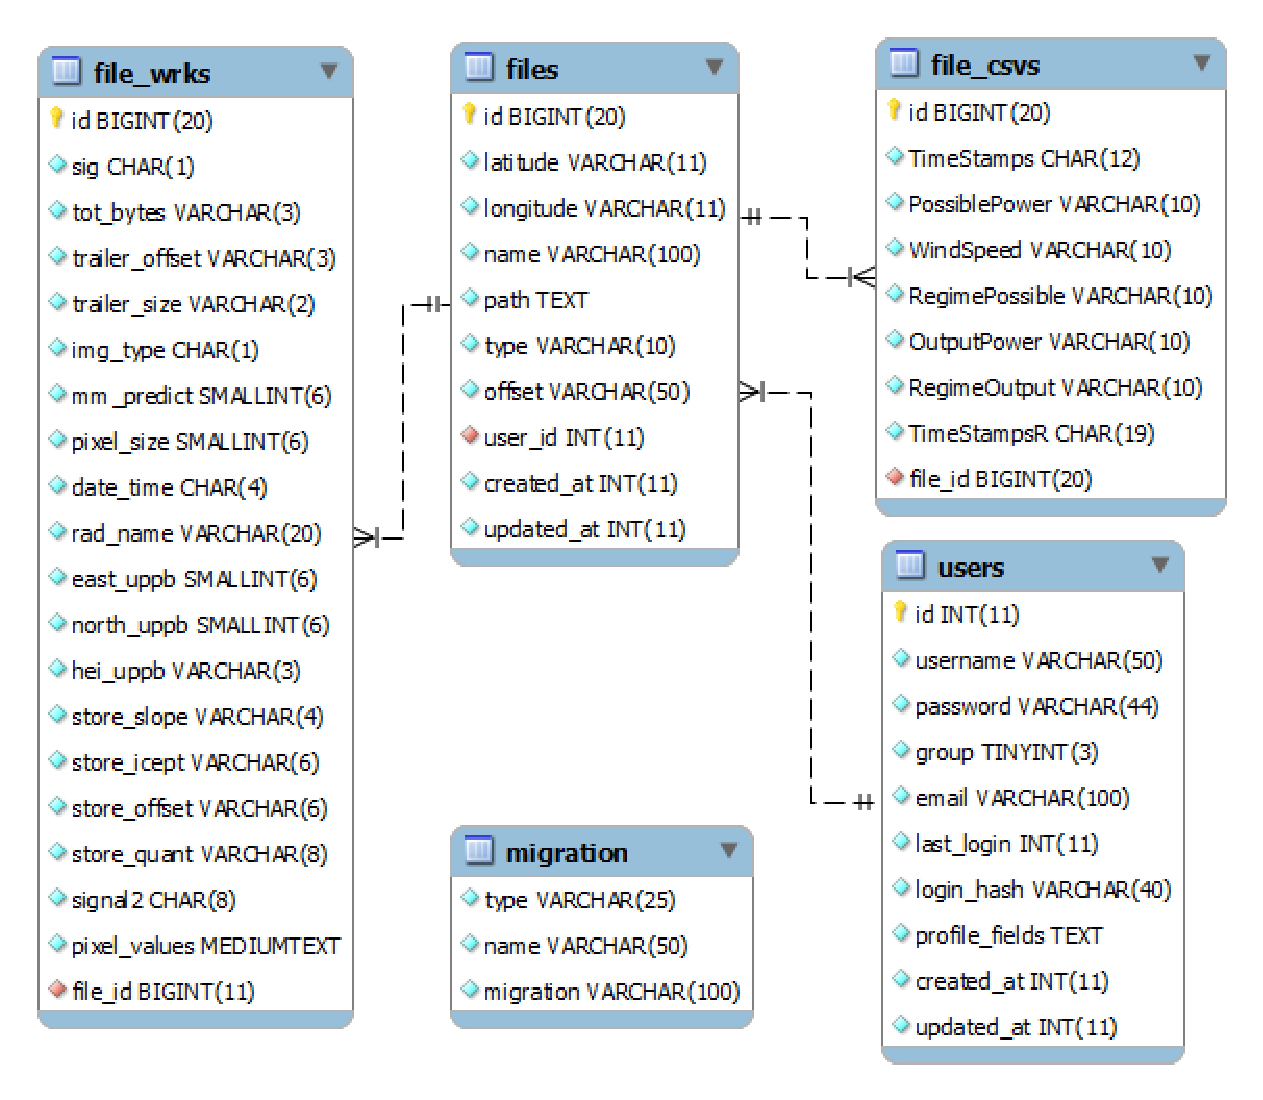
\includegraphics[width=1\linewidth]{figure/db}
   \caption{Database Diagram}
   \label{fig:dbdiagram}
\end{figure}

FuelPHP contains a \textsf{migration} tool that lets one create revisions for the database, hence easy deployment of changes. This tool has been used to create all tables, and therefore the \textsf{migration} table is used to keep track of revisions.

All tables use \textsf{InnoDB}, because this engine make it possible to create sql relations. This means that if a table has a foreign key (i.e. a key that identifies a row in another table), one can create actions for what should happen to the rows in the current table, if the related row in the other table is \textsf{updated} or \textsf{deleted}.

These relations can be seen in the diagram. The relations and actions is stated by sql as in listing \ref{lst:sql}
\begin{lstlisting}[language=sql,caption={SQL realations and actions},label={lst:sql}]
ALTER TABLE `files`
  ADD CONSTRAINT `files_ibfk_1` FOREIGN KEY (`user_id`) REFERENCES `users` (`id`) ON DELETE NO ACTION ON UPDATE NO ACTION;

ALTER TABLE `file_csvs`
  ADD CONSTRAINT `file_csvs_ibfk_1` FOREIGN KEY (`file_id`) REFERENCES `files` (`id`) ON DELETE CASCADE ON UPDATE NO ACTION;

ALTER TABLE `file_wrks`
  ADD CONSTRAINT `file_wrks_ibfk_1` FOREIGN KEY (`file_id`) REFERENCES `files` (`id`) ON DELETE CASCADE ON UPDATE NO ACTION;
\end{lstlisting}

\subsection{Optimization}
\label{sec:database_optimization}
In FuelPHP it is possible to create model relations that are similar to sql relations with actions, but easier to manage and at the same time less efficient (though generally adequate). This method was used initially, but performance was found to be too bad, e.g. it would take too much time to cascade delete all the csv rows related to the file selected for deletion, eventually leading to a time out by the server. The time out limit can be changed by the server manager, but it was easier and - as stated before - more efficient to make relation actions in sql. Relations are still present at model level, but actions have been turned off.

When first creating the database, the data types for the fields were not optimized, and as previously stated this is important for performance, and improper data types or constraints can even break the data that should be saved. When optimising the data types, we were also able to gain space and e.g. halve the size of the \textsf{file\_csvs} from maximum 372 bytes per row to maximum 107 bytes.

As seen on figure \ref{fig:dbdiagram}, \textsf{id} for  \textsf{files, file\_csvs} and  \textsf{file\_wrks} are of type \textsf{bigint} ( \textsf{unsigned}). This make it possible for these tables to store a huge amount of data, and even though \textsf{unsigned int} can save a large amount too, we would rather make the application future proof than let it break if the limit was reached.

Equations \ref{eq:db_1} through \ref{eq:db_4} illustrate the problem and reason for the decision made.

\emph{Number of csv files stored, if the data is represented by a 10 minute interval in a span of 1.5 years (as current test data):}

\textsf{unsigned int}: 
\begin{equation}
\label{eq:db_1}
\left\lfloor \frac{2^{32}-1}{72,858} \right\rfloor = 58,949
\end{equation}

\textsf{unsigned bigint}:
\begin{equation}
\label{eq:db_2}
\left\lfloor \frac{2^{64}-1}{72,858} \right\rfloor = 253,187,626,255,312
\end{equation}

\emph{Number of csv files stored, if the data is represented by a 1 minute interval in a span of 1.5 years:}

\textsf{unsigned int}:
\begin{equation}
\label{eq:db_3}
\left\lfloor \frac{2^{32}-1}{72,858 \cdot 10} \right\rfloor = 5,894
\end{equation}

\textsf{unsigned bigint}:
\begin{equation}
\label{eq:db_4}
\left\lfloor \frac{2^{64}-1}{72,858 \cdot 10} \right\rfloor = 25,318,762,625,531
\end{equation}

As the storage size of \textsf{bigint} is only twice as big as \textsf{int}, the maximum increase in storage per row is not remarkable, where as the increase in number of possible files storeable is increased by a huge margin as seen on equation \ref{eq:db_3} and \ref{eq:db_4}.

% api.tex should start at section level
\section{API}
The application has a small API\footnote{Application programming interface} that the application it self uses to retrieve some of the data.

\subsection{Radars}
A list of images for a radar can be retrieved by calling
\begin{lstlisting}[language=sh]
GET http://WEBROOT/rest/radar/list.TYPE?lat=LAT&lng=LNG&f=FROM
\end{lstlisting}
Where \textsf{WEBROOT} is the domain name of the server, \text{TYPE} is the return type\footnote{All formats supported by FuelPHPs REST controller is supported. A list of supported formats can be found at \url{http://docs.fuelphp.com/general/controllers/rest.html\#/formats}.\label{fn:fuel_rest}}, \textsf{LAT} is the latitude of the radar, \textsf{LNG} is the longitude of the radar and \text{FROM} is a date from which the data should start from.

The returned data is in array format, where each element is an array consisting of two elements. The first is the timestamp of the image, and the second is the url of the radar image relative to the \textsf{WEBROOT}.

\subsection{Wind farms}
A list of data from a given wind farm can be retrieved by calling
\begin{lstlisting}[language=sh]
GET http://WEBROOT/rest/csv/list.TYPE?id=ID&c=COL&f=FROM&t=TO
\end{lstlisting}
Where \textsf{WEBROOT} is the domain name of the server, \textsf{TYPE} is the return type\footref{fn:fuel_rest}, \textsf{ID} is ID of the wind farm, \textsf{COL} is the column\footnote{Currently \textsf{PossiblePower}, \textsf{OutputPower}, \textsf{WindSpeed}, \textsf{RegimePossible} and \textsf{OutputRegime}. Note that the columns are case-sensitive.} to fetch data from, \text{FROM} is a date from which the data should start from and \text{TO} is a date at which the data stops at.

The returned data is in array format, where each element is an array consisting of two elements. The first is the timestamp of the image, and the second is the url of the radar image relative to the \textsf{WEBROOT}.

\subsection{Jobs}
A number of files currently in queue to be parsed can be retrieved by calling
\begin{lstlisting}[language=sh]
GET http://WEBROOT/rest/jobs/list.TYPE
\end{lstlisting}
Where \textsf{WEBROOT} is the domain name of the server.

\subsection{Upload}
It is possible to send data to the application, just as if they were being uploaded manually. This allows for remote services to send `real time' data to the application. To send data to the server, the following call should be made:
\begin{lstlisting}[language=sh]
curl -F "path=@FILE" http://WEBROOT/api/upload -H "X-KEY: KEY=" -H "X-TIMEZONE: ZONE" -X POST
\end{lstlisting}
Where \textsf{FILE} is the path to the file on the senders machine, \textsf{WEBROOT} is the domain name of the server, \textsf{KEY} is an API key and \textsf{ZONE} is the time zone given by MySQLs Zoneinfo\footnote{See section \ref{sec:application_requirements} for notes about installation of Zoneinfo}.

An example call, to upload \textsf{ekxr20101218\_2350.wrk} with UTC timestamps to the \textsf{WEBROOT} server with the default admin user woudl look like this:
\begin{lstlisting}[language=sh]
curl -F "path=@ekxr20101218_2350.wrk" http://WEBROOT/api/upload -H "X-KEY: YWqmPGH+dOEvOh6pf83a62lzJ1QQLHRMPHhNIaohB3s=" -H "X-TIMEZONE: UTC" -X POST
\end{lstlisting}



\section{Radar annotation}
In the final stages of the application, it was discussed if radars should have its name and/or time stamp for the current radar image shown to make it clearer for the user when the image was taken.

Figure \ref{fig:mock_up_inactive_radar} and \ref{fig:mock_up_active_radar} shows the mock ups for the radar in both inactive and active state.
\begin{figure}[htbp]
  \begin{minipage}[b]{0.5\linewidth}
    \centering
    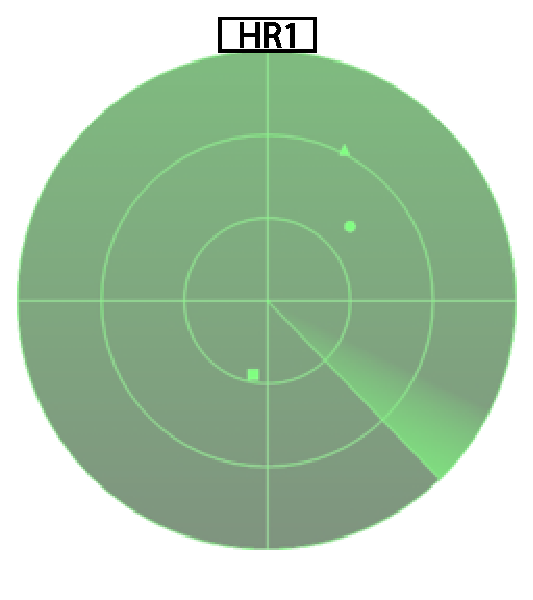
\includegraphics[width=\linewidth]{figure/radar1.eps}
    \caption{Mock up of inactive radar}
    \label{fig:mock_up_inactive_radar}
  \end{minipage}
  \hspace{0.5cm}
  \begin{minipage}[b]{0.5\linewidth}
    \centering
    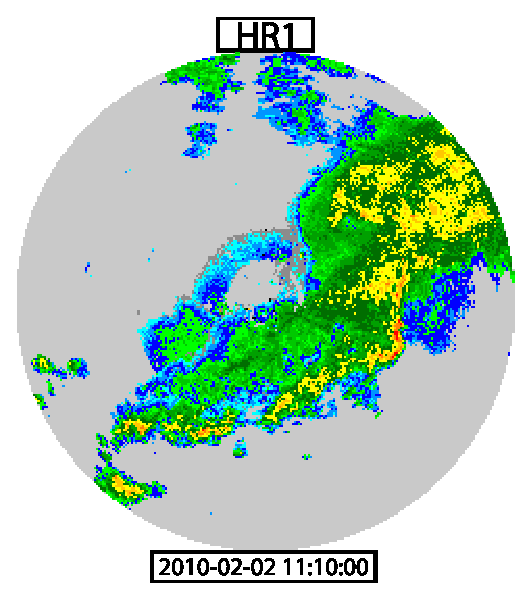
\includegraphics[width=\linewidth]{figure/radar2.eps}
    \caption{Mock up of active radar}
    \label{fig:mock_up_active_radar}
  \end{minipage}
\end{figure}
The added name and time stamp might pose as a problem, if two radars were placed in such a way that their range would overlap where the name or time stamp were put.

This could be somewhat solved, by fading out the radars too close to an active radar, in the same way that windmills inside the range of a radar is faded out when a radar animation starts.

\section{Data date range}
As time goes by, one would expect the application to contain massive amounts of data.
In the provided test data\footnote{Data02122.tar.gz provided by Pierre-Julien Trombe on CampusNet}, the application contains \textasciitilde 140 rows of data for \textsf{wrk} files and \textasciitilde 73,000 rows of data for the wind farm data.

It was discussed how we should limit the view of data, since it would require quite a lot of processing power to display that much data.

For the wind farm chart, we went from 1-month, weekly and daily view to 2-week, weekly and daily.
Preliminary tests showed that the loading time for 1-month view was too slow, because of the huge amount of data that had to be processed and formatted correctly before sent to the browser. The data would also take long to download, especially if not on a high speed internet connection.

Another problem was the radar images. Without any data range, they would all start at the first image taken by that radar, and play till the last. A range chosen by the user from a `to' and `from' date field was suggested. After testing the first implementation it was found that the `to' field was a bit confusing and would result in a bit of a rewrite of already existing code.

The `to' field was removed and the `from' field now decides the starting date for all radars and wind farm charts.
All radars will start their animation on the first image taken after the selected from date.
The chart will also start at the selected start date, but the navigation buttons allows one to go either back or forth in time independent of the selected from date.

\section{The data}
\subsection{Implementation}
After the implementation of wrk files, it was discussed whether or not the NetCDF should be implemented and it was decided that the time cost were too big to meet the deadline. Instead it was concluded that the flexibility of the application was good enough to allow extending the application to support other file formats, including NetCDF, at a later date and the focus was shifted to the frontend.

\subsection{Grouping wrk}
The big amount of wrk files for each radar (1 every \textasciitilde 10 minutes for a total of 144 files per day) causes a bit of confusion in the file administration of the control panel.

It was suggested that the administration panel grouped the wrk files per day, or that the data parser combined one day of wrk files into one file before importing it into the database.

The idea of letting the data parser to handle the merge was dropped due to the complexity. A merge in the data parser would also increase the memory usage by the data parser, which might not be available on the web server running the application.

Lack of time prevented the implementation of file grouping by the administration panel because of the work involved in finding the files that should be grouped together.

\subsection{Choice of map}
After comparing the two maps, it quickly became OpenStreetMap. It was partly because of Google wants money if the map is used for commercial purposes and because the data is copyrighted and owned by multiple organisations. This wasn't the way we were thinking about open source.

OpenStreetMap wasn't that difficult to work with, due to the very well documentation from leaflet\footnote{See \cite{leaflet} for the documentation}.

There have been several design ideas. Many changes through the project and many considerations.

\subsubsection{Map}
At the beginning we had a sidebar which could be visible or hidden (figure \ref{fig:map_v1}). Later we found out that there is no need for a big menu, so we removed the sidebar and added a tiny top bar, with only the necessary options.\\
First mockup:
\begin{figure}[htbp]
   \centering
   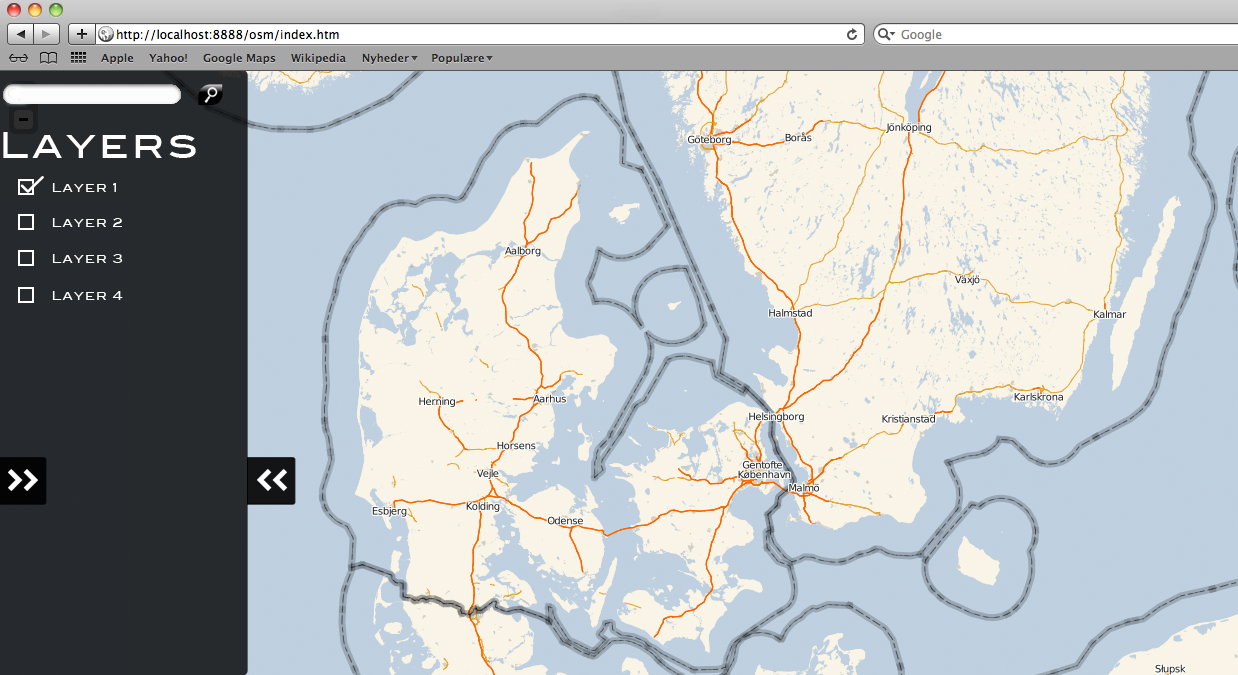
\includegraphics[scale=.3]{figure/design_map_v1.eps}
   \caption{Map - version 1}
   \label{fig:map_v1}
\end{figure}

We would like to have different layers on the map at the beginning, but this was unnecessary, so it was quickly removed.\\
Now we have created a cool design which is easy to get used to and all relevant informations can be accessed easily and without to much clicking (figure \ref{fig:map_final}).
There have also been added some gestures to control the radar easily.\\
The top bar has a date field to know which date the radar should get data from. This date will be transferred to the chart window.

\begin{figure}[htbp]
   \centering
   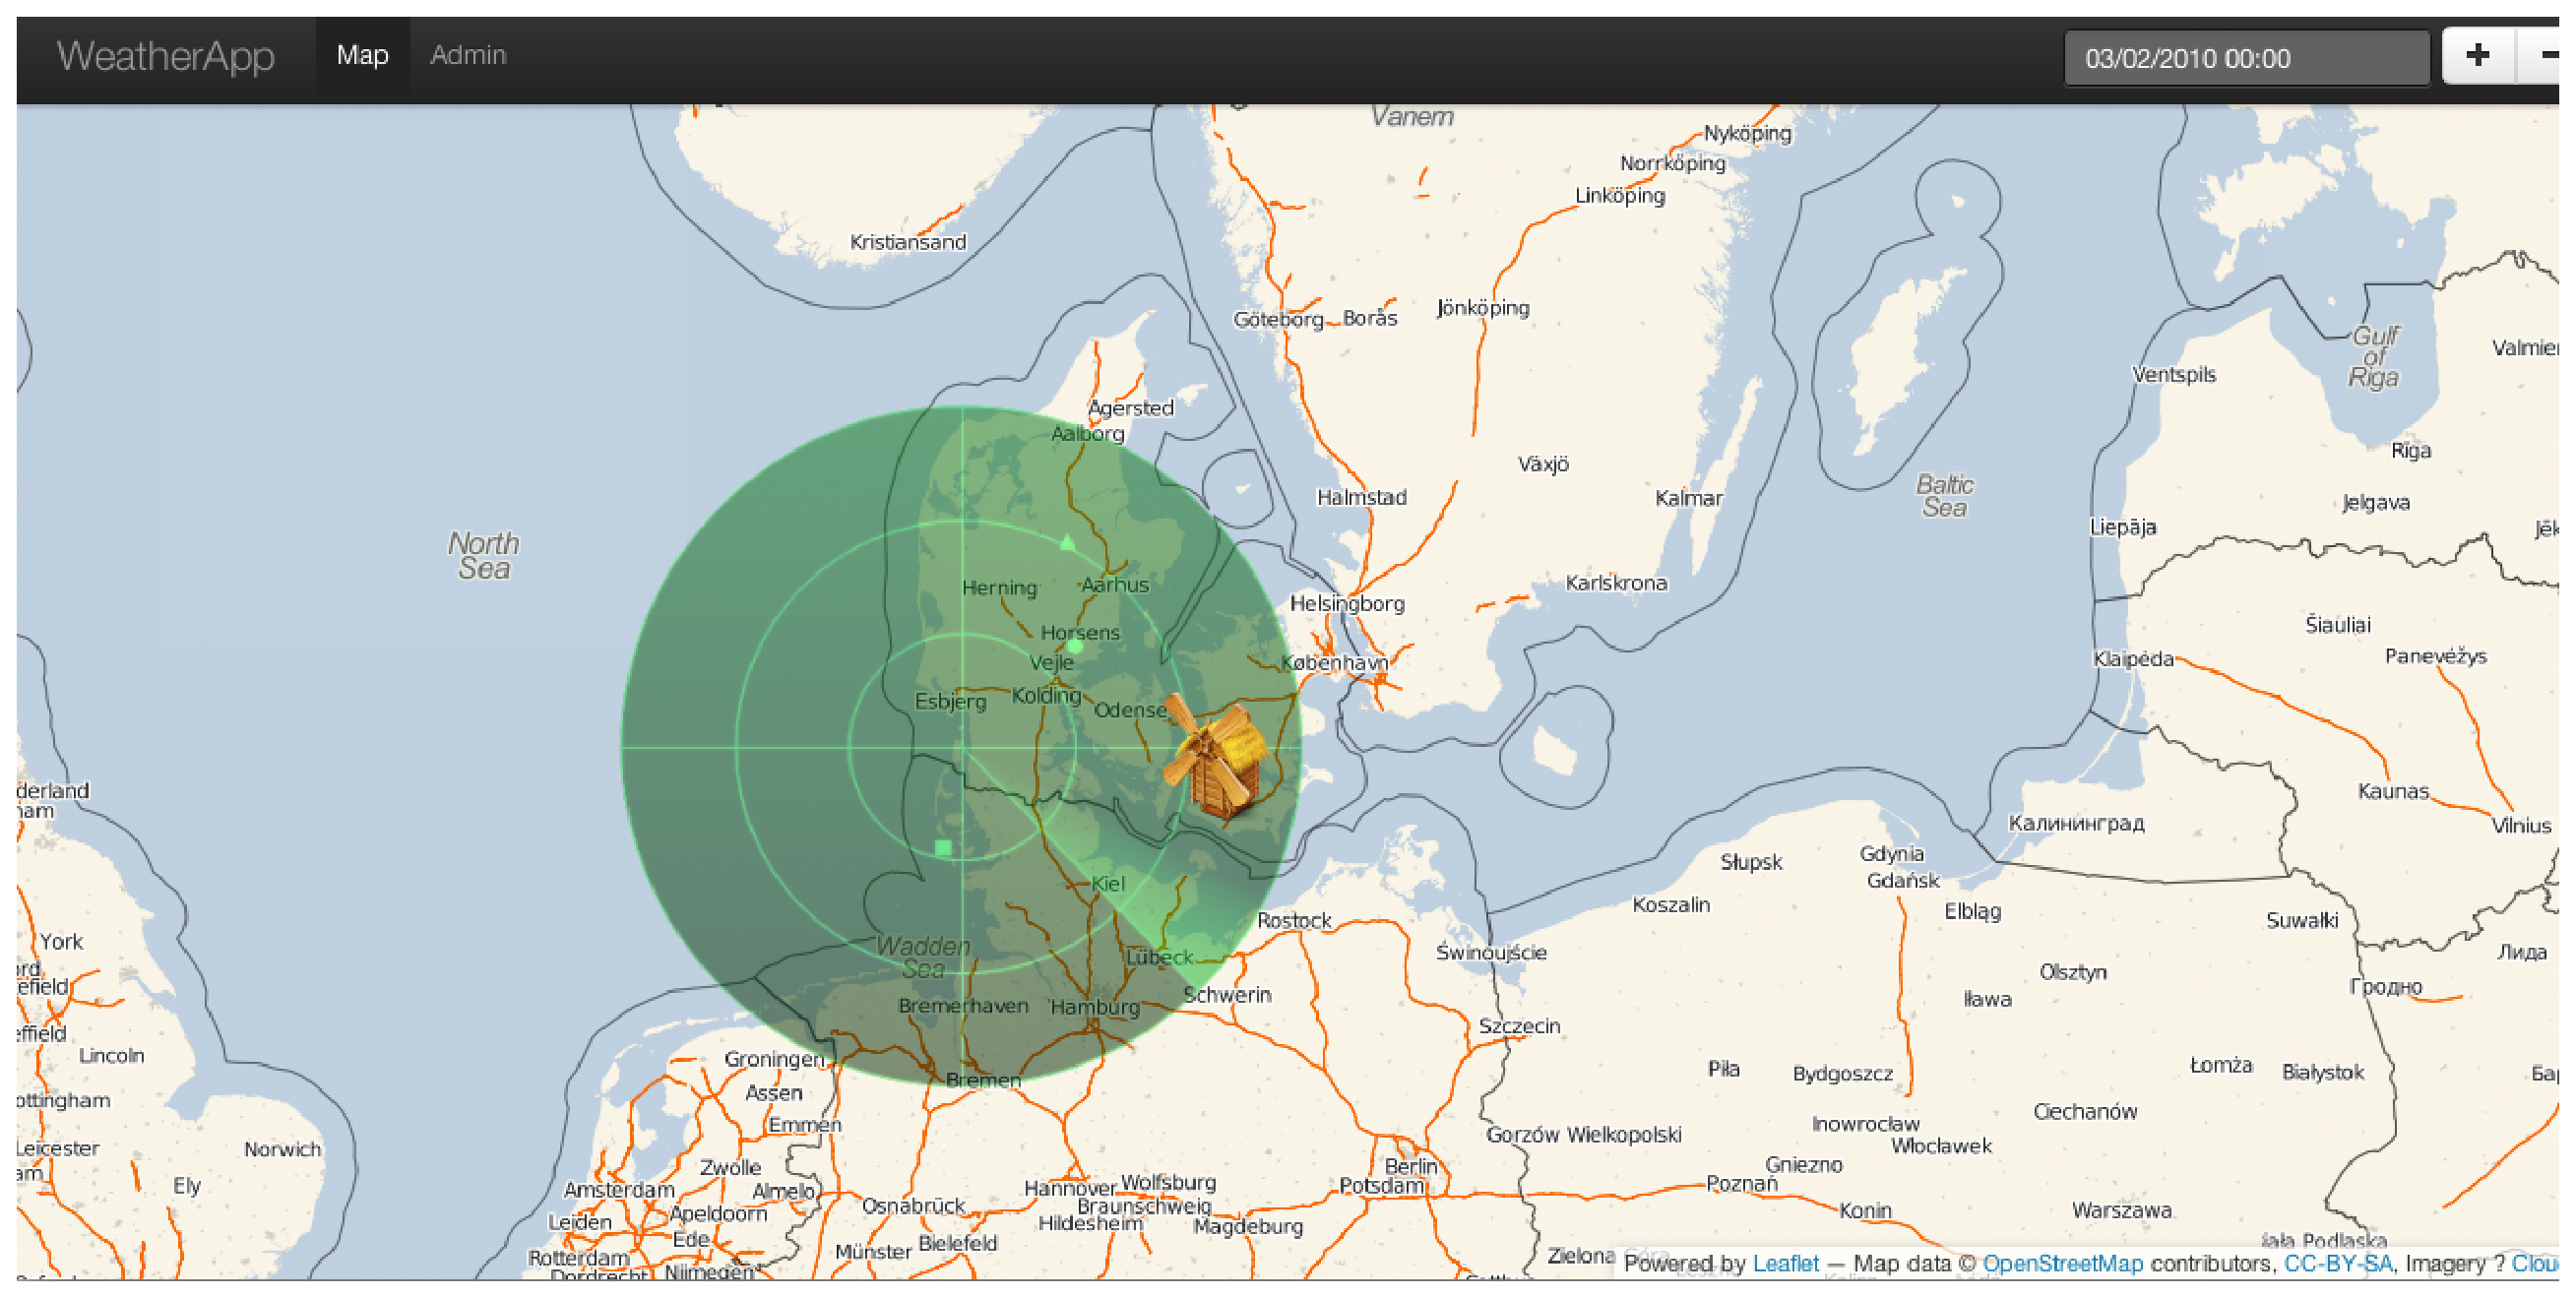
\includegraphics[width=1\linewidth]{figure/design_map_final.eps}
   \caption{Map - final}
   \label{fig:map_final}
\end{figure}

\subsubsection{Chart}
At the beginning we had the same sidebar as on the map, but with other options (figure \ref{fig:chart_v1}). This was also replaced by a top bar like on the map.\\
First mockup: 
\begin{figure}[htbp]
   \centering
   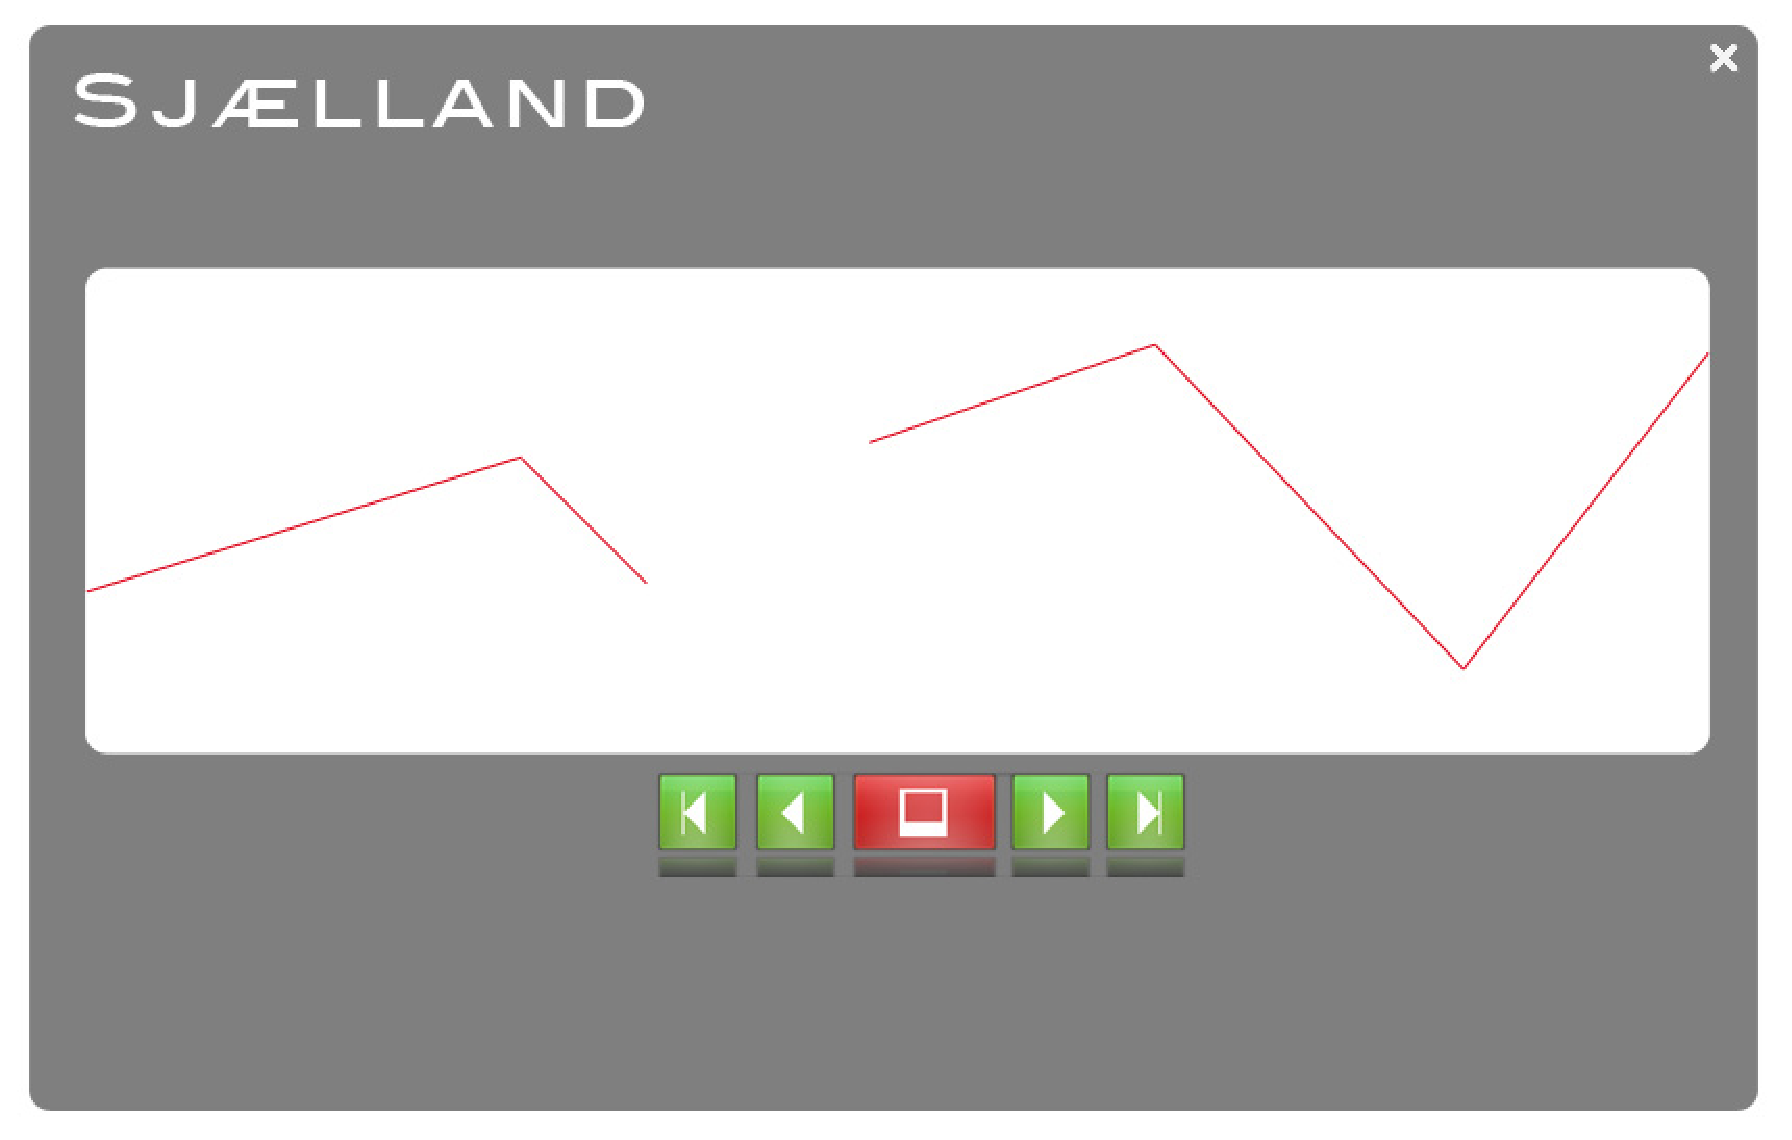
\includegraphics[width=1\linewidth]{figure/design_chart_v1.eps}
   \caption{Chart pop up - version 1}
   \label{fig:chart_v1}
\end{figure}

This has, through the whole project, been determined to be a pop up on the map.
The control buttons were before 'fast backward', 'backward', 'today', 'forward' and 'fast forward', but 'today' was replaced with 'play'. The 'play' button moves the chart every second, so the user can view the chart animated.\\
The new design also have three different views '2-week', 'weekly' and 'daily view' (figure \ref{fig:chart_final}). Control buttons adjust to the view the user has selected.

\begin{figure}[htbp]
   \centering
   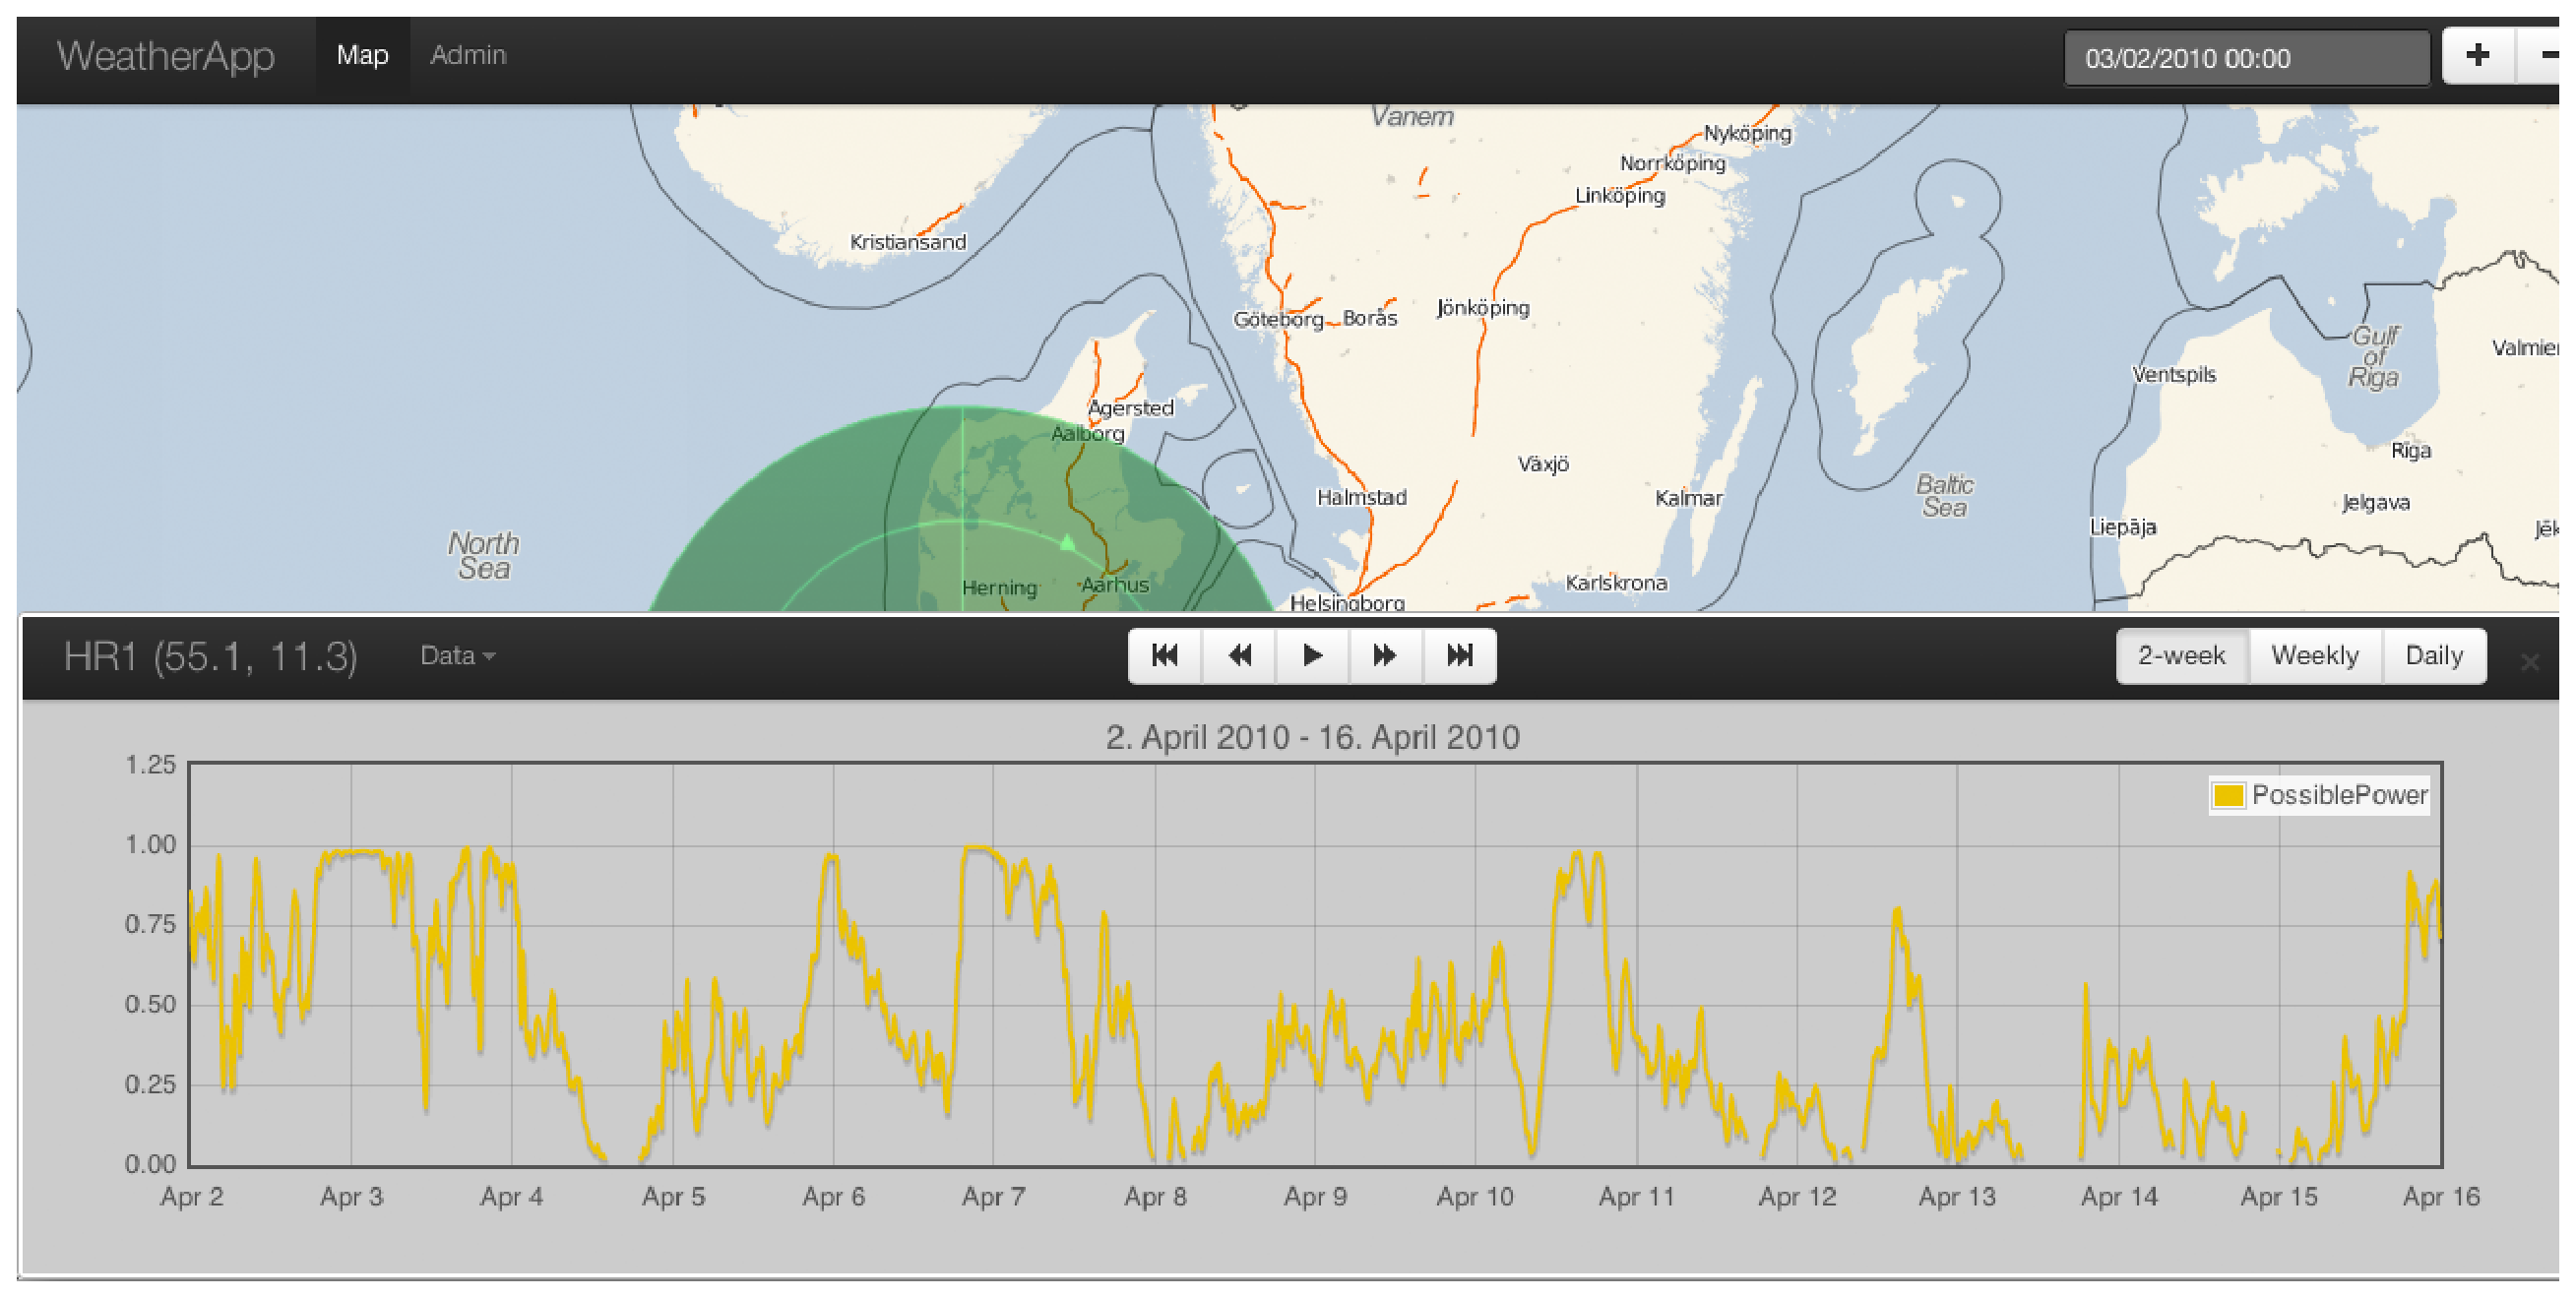
\includegraphics[width=1\linewidth]{figure/design_chart_final.eps}
   \caption{Chart pop up - final}
   \label{fig:chart_final}
\end{figure}

\chapter{Restrictions and limitations}
\label{sec:restrictions_and_limitations}
Under the development of the application, a few assumptions have been made, and have resulted in the following restrictions and limitations by design.

For the radar images to display properly, the values of \textsf{east\_uppb} and \textsf{north\_uppb} will have to be equal in the \textsf{wrk} files, which they really ought to.

The range of the radar is calculated from \textsf{east\_uppb} and \textsf{pixel\_size}, which underlines the need for the radar image to be a perfect square.

All users have a limit on the size of the username on 50 characters and 100 characters for the email.
Also, all usernames and passwords \textbf{has} to be at least 3 characters long.

Time zone names is limited to 50 characters. Should the time zone names from zoneinfo\footnote{See section \ref{sec:application_requirements} on info about zoneinfo} exceed 50 characters, the limit can be increased by altering the database column and changing the constraint in the file model.

\section{Known issues}
\label{sec:known_issues}
This chapter is dedicated to highlight the known issues in the application that were not resolved due to lack of time.
\begin{itemize}
\item Due to the reset feature implemented on the radars, the windmills might do more fade in and outs than intended if the radar is clicked before an animation has finished.
This could be resolved by adding a check to see if an animation is in progress, before queuing a new one.
\item When viewing a chart, it is possible to scroll to a date that is newer than the last data of that wind farm. A check should be implemented and inform the user that the wind farm does not have any more data.
\item No versions of Internet Explorer is supported, so the application might or might not work as intended in that browser. Mozilla Firefox or Google Chrome is recommended. See section \ref{sec:cross-platform} for more info.
\item If a file is uploaded with the same name as one that already exists on server, the file is skipped.
\end{itemize}
\chapter{Application requirements}
\label{sec:application_requirements}
The application requires a few things in order to run.

\section{Server side}
\begin{description}
\item[Web server] A web server is needed in order to run the web site. It is also required to have permissions to run executables. The included data parser is compiled for Windows, OSX and Ubuntu. If the web server is not allowed to run the included executables, they should be ran as a CGI script - This has not been tested however.
\item[PHP] The web server should support PHP version 5.3+.
\item[GD] The application uses GD 2.0.1+ (2.0.28+ is recommended) to create radar images.
\item[MySQL] FuelPHP supports multiple databases through drivers, but in order to support time zones correctly, we've chosen to take advantage of MySQLs own methods. This means that MySQL 5.5.20+ is required.
\item[Zoneinfo] MySQL needs Zoneinfo in order for the time zones to work properly\footnote{On linux, the following command can be executed in the terminal to import zoneinfo: \mbox{\textsf{> mysql\_tzinfo\_to\_sql /usr/share/zoneinfo | mysql -u root -p mysql}}. Other operating systems might not have the zoneinfo, and will have to download it from \url{http://dev.mysql.com/downloads/timezones.html} and import it to the mysql database.}
\item[Safe mode] Safe mode might need to be disabled in the PHP configuration, if \textsf{fopen}\footnote{See \url{http://php.net/manual/en/function.fopen.php}.} is not allowed to access some files.
\end{description}

\section{Client side}
\begin{description}
\item[JavaScript] It is required that the users browser supports and has enabled JavaScript in order for the site to work.
\end{description}
\chapter{Work flow \& distribution}
At the beginning Dropbox\footnote{A web based file hosting service - see \cite{Dropbox}} was used to sharing files between group members, using a shared folder, all members could read and write to. It was fine at the beginning, but later when there became file conflicts , it started to get a little problematic, since Dropbox doesn't have a smart merging algorithm.
There was created a public repository at Git\footnote{A web based hosting service - see \cite{Git}} to push and pull data to the git server, so files could be changed without to many conflicts. Git was used, because of the merging algorithm and easy to use.

Git allows you to view older files and list commits\footnote{Every time a person push data to Git, he also gives a comment of what he has done. In that way it is easier to get an overview of changes.} from users through the whole project.

Git also allow other users to look at the program and and test it by them self, so it is accessible for all.

Since Git is used, everyone can access the repository\footnote{Repository \url{http://github.com/connors511/WeatherDataVisualization}} by them self. Users can't change or commit data, but can download the application and give comments to the project.

\section{Distribution}
As this software project have been carried out by a group, we have been working together as a team with constructive criticism of each other, spelling and syntax correction ect. This means that everyone have more or less had a hand in every part of the software. However:

Mads Lundt have had the main responsibility of the following parts of the software:
\begin{itemize}
\item Map (HTML + JavaScript)
\end{itemize}

Matthias Larsen have had the main responsibility of the following parts of the software:
\begin{itemize}
\item Data Parser (C++)
\end{itemize}

Joachim Jensen have had the main responsibility of the following parts of the software:
\begin{itemize}
\item File upload (PHP)
\end{itemize}
\chapter{Conclusion}
There was created a weather application, that met the requirements we stated at the beginning.
It was not easy, since there are no applications with our specified requirements, that could inspire us.

The implementation of different file types, data visualizing and database integration, to make it easier and to get higher performance, are completed in that way it was required from the beginning. While there is a lot of focus on extensibility and simplicity.
 
The implementation that did not finish, were the NC-files, due the troubles with CSV and WRK. This and coordinates converting were not implemented, due there was no test data with other coordinates, but as earlier stated, this can be implemented.

The use of Git was much better than Dropbox, that was used in the beginning, and allowed all group members to change files without too much concern for conflicts.

The final product ended up being a satisfied solution for a weather application, that could analyze and visualize the enormous amounts of data in an intuitive way.
\chapter{Future work}

Besides fixing the currently known bugs stated in BUGS REFERENCE, we have some ideas for the application, some of which have been described in ANALYSE REFERENCE that did not make it to the existing application.

\section{GPS coordinates}
There are several ways to locate positions on a map. We have used \emph{conjugate graticule}\footnote{Latitude/Longitude also known as conjugate graticule}, because the test data we had available used this. We haven't implemented for other GPS coordinates than latitude and longitude, because of the time pressure.

We know that there are other methods to get GPS coordinates - one of them is \emph{Degrees, Minutes, Seconds}. In a circle there are 360 degrees, so to get a minute each degree is split up into 60 parts, \nicefrac{1}{60}th of a degree. To get seconds each minute is split up into 60 parts, \nicefrac{1}{60}th of a minute.

To convert \emph{Degrees, Minutes, Seconds} into latitude and longitude, just simply use the formula:
\begin{equation}
Degrees~ + \left(Minutes~ \cdot \nicefrac{1}{60}\right) + \left(Seconds~ \cdot \nicefrac{1}{60} \cdot \nicefrac{1}{60}\right)
\end{equation}

Converting the other way around should be a bit more difficult, but since openstreetmap is using latitude and longitude, this isn't necessary.


%%%%%%%%%%%%%%%%%%%%%%%%%%%%%%%%%%%%%%%%%%%%%%%%%%%%%%%%%%%%%%%%%%

%%%%%%%%%%%%%%%%%%%%%%%%%%%%%%%%%%%%%%%%%%
% BIBLIOGRAPHY: Build - bibtex to renew
%	\clearpage{\thispagestyle{empty}\cleardoublepage} \phantomsection 
%	\ifx\thesislanguage\danishlang
%	\addcontentsline{toc}{chapter}{Litteratur}
%	\else
%	\addcontentsline{toc}{chapter}{Bibliography}
%	\fi
%	\bibliographystyle{plainnat}
%\bibliography{bibbase}

%% Ad to Runin headings:
	\ifx\thesislanguage\danishlang
	\markboth{Litteratur}{}
	\else
	\markboth{Bibliography}{}
	\fi
%%%%%%%%%%%%%%%%%%%%%%%%%%%%%%%%%%%%%%%%%%

%%%%%%%%%%%%%%%%%%%%%%%%%%%%%%%%%%%%%%%%%%%%%%%%%%%%%%%%%%%%%%%%%%
% REFERENCE:
\clearpage{\thispagestyle{empty}\cleardoublepage} \phantomsection 
\addcontentsline{toc}{chapter}{References}
\renewcommand\bibname{References}
\bibliographystyle{plain}
\begin{thebibliography}{10}
\bibitem{VRIS}
\emph{Vejrradar informations System}.
see \texttt{Dmi\_file\_format\_description.pdf}, section `The new VRIS format'.

\bibitem{wikiBMP}
\emph{Microsoft Windows Bitmap Format}.
\url{http://en.wikipedia.org/wiki/BMP_file_format}

\bibitem{leaflet}
\emph{OpenStreetMap Leaflet documentation}.
\url{http://leaflet.cloudmade.com}

\bibitem{jquery}
\emph{jQuery documentation}.
\url{http://docs.jquery.com}

\bibitem{GPS}
\emph{Global Positioning System}.
\url{http://en.wikipedia.org/wiki/Global_Positioning_System}

\bibitem{dropbox}
\emph{Dropbox}.
\url{http://dropbox.com}

\bibitem{git}
\emph{Git}.
\url{http://github.com}
\end{thebibliography}

%%%%%%%%%%%%%%%%%%%%%%%%%%%%%%%%%%%%%%%%%%%%%%%%%%%%%%%%%%%%%%%%%%

%%%%%%%%%%%%%%%%%%%%%%%%%%%%%%%%%%%%%%%%%%%%%%%%%%%%%%%%%%%%%%%%%%
% APPENDIX:
\clearpage{\thispagestyle{empty}\cleardoublepage} \phantomsection 
	\appendix	
	\ifx\thesislanguage\danishlang
	\addcontentsline{toc}{chapter}{Appendiks}
	\else
	\addcontentsline{toc}{chapter}{Appendix}
	\fi
%\chapter{Appendix}
%\label{ap:benchmark}
%\lstinputlisting[language=c,caption={benchmark.h},label=benchmark.h]{./appendix/benchmark.h}
%\lstinputlisting[language=c,caption={benchmark.c},label=benchmark.c]{./appendix/benchmark.c}

\chapter{CSV Definition}
\label{ap:csv}
The wind farm data is of the file type csv. The file can be split up into 2 pieces.
\section{The header}
The header consists of two lines. The first line defines the latitude, longitude and the name of the wind farm from which the data originates.
The second line defines the columns, which \textbf{has} to be the same as shown in listing \ref{ap:ex:csv}.

\section{The body}
The third and following lines contains the data itself.

\section{Template}
\lstinputlisting[language=sql,caption={CSV template},label=ap:ex:csv]{./appendix/template.csv}

\chapter{Use cases}
\label{ap:usecase}
We have two types of actor:
\begin{itemize}
\item User: Ordinary person.
\item Admin: User with permission to access administration.
\end{itemize}

\section{Clicking on a radar at the map}
\textbf{Actor:} User

\textbf{Scenario:}
\begin{itemize}
\item Checks if there is data for the date
\item If images isn't generated, it will generate them real time.
\item Radar shows images over an interval.
\item \emph{One click for play/pause and doubleclick for reset.}
\item When there is no more data, the radar resets.
\end{itemize}
\textbf{Alternative scenario:} 
\begin{enumerate}
\item No data is available for that moment and a message appears.
\end{enumerate}

\section{Clicking on a wind farm at the map}
\textbf{Actor:} User

\textbf{Scenario:}
\begin{itemize}
\item Visualize data for that given wind farm.
\end{itemize}

\section{Changing view in chart for wind farm}
\textbf{Actor:} User

\textbf{Scenario:}
\begin{enumerate}
\item Changing to 2-week view.
\begin{itemize}
\item Changing chart view interval to 2 weeks.
\item Load new data for the new interval.
\end{itemize}
\item Changing to weekly view.
\begin{itemize}
\item Changing chart view interval to 1 week.
\item Load new data for the new interval.
\end{itemize}
\item Changing to daily view.
\begin{itemize}
\item Changing chart view interval to 1 day.
\item Load new data for the new interval.
\end{itemize}
\end{enumerate}

\section{Changing data to be shown}
\textbf{Actor:} User

\textbf{Scenario:}
\begin{itemize}
\item The data is shown.
\end{itemize}
\textbf{Alternative scenario}
\begin{enumerate}
\item The data is removed.
\end{enumerate}

\section{Using control buttons in chart for wind farm}
\textbf{Actor:} User

\textbf{Scenario:}
\begin{enumerate}
\item Pressing fast backward.
\begin{itemize}
\item Go two weeks back on 2-week view, one week back on weekly view and one day on daily view.
\item Loads new data.
\end{itemize}
\item Pressing backward.
\begin{itemize}
\item Go one week back on 2-week view, one day back on weekly view and one hour on daily view.
\item Loads new data.
\end{itemize}
\item Pressing play.
\begin{itemize}
\item Change to daily view and go one hour forward every second.
\item Loads new data.
\end{itemize}
\item Pressing forward.
\begin{itemize}
\item Go one week forward on 2-week view, one day forward on weekly view and one hour on daily view.
\item Loads new data.
\end{itemize}
\item Pressing fast forward.
\begin{itemize}
\item Go two weeks forward on 2-week view, one week forward on weekly view and one day on daily view.
\item Loads new data.
\end{itemize}
\end{enumerate}

\section{Upload file}
\textbf{Actor:} Admin

\textbf{Scenario:}
\begin{itemize}
\item Sign in with correct username and password.
\item Add new file (CSV, WRK, ZIP) and enter correct timezone.
\item If file is ZIP, it will decompress.
\item File is uploaded.
\item File is being parsed.
\end{itemize}
\textbf{Alternative scenario:} 
\begin{enumerate}
\item Sign in with wrong username or password.
\item Adding file that isn't correct format and get an error message.
\item Adding ZIP file, but files inside zip isn't correct. It will get an error message.
\item File exists and will not be uploaded.
\end{enumerate}

\chapter{Installation}
\label{ap:installation}
\chapter{Installation}

In the following it is implied that the chosen solutions for each step - e.g. if more than one option is possible - are compliant with the TECHNICAL REQUIREMENTS.

\begin{enumerate}
\item Download the source from \url{https://github.com/connors511/WeatherDataVisualization} in \textsf{/application}.
\item Set up a webserver to host the application, either locally or on the World Wide Web.
\item Create a database and set the connection information in \textsf{App/fuel/config/development/db.php}
\item Create the database tables. This can be done by running the following with \textsf{Oil} in command line:
\begin{lstlisting}[language=sh]
php oil g r migrate
\end{lstlisting}
\item Log in to the application with username/password: \textsf{admin/admin}.
\end{enumerate}

%%%%%%%%%%%%%%%%%%%%%%%%%%%%%%%%%%%%%%%%%%%%%%%%%%%%%%%%%%%%%%%%%%

\label{fancy:mainend} %for 'of page /x'
\clearpage{\thispagestyle{empty}\cleardoublepage}

%%%%%%%%%%%%%%%%%%%%%%%%%%%%%%%%%%%%%%%%%%
% BACK MATTER:
	\backmatter
	\ifx\thesisversion\printversion
	\makebackpage %generates the backmatter (thesislayout.sty)
	\fi
%%%%%%%%%%%%%%%%%%%%%%%%%%%%%%%%%%%%%%%%%%

\end{document}